\subsection{Overview}
This chapter outlines the four-layered architecture of the Best Bike Paths (BBP) system. We begin by mapping the high-level tiers and their primary communication paths. This is followed by an exploration of the individual components and their specific functional responsibilities. The document then describes the deployment strategy and the runtime dynamics between components, including a formal definition of their interfaces. Finally, we discuss the design patterns and strategic choices implemented to ensure the system meets its scalability and fault-tolerance objectives.

\subsubsection{System View}

The Best Bike Paths (BBP) platform is organized into a four-tier architecture consisting of a presentation tier, web-tier, business-tier and a dedicated data tier. The presentation tier handles user interactions, sensor data acquisition and communication with the map service, while the web tier handle the interaction between the presentation and the business tier, and it includes an external proxy for API calls to the weather service. The web server manages HTTPS requests from the presentation tier and routing internal requests to the business tier, while the business tier hosts the core logic of the application, and the data tier includes the database server. To ensure high availability and resilience, all components are designed for replication and container-based deployment, effectively preventing single points of failure across the system.

\begin{figure}[!h]
    \centering
    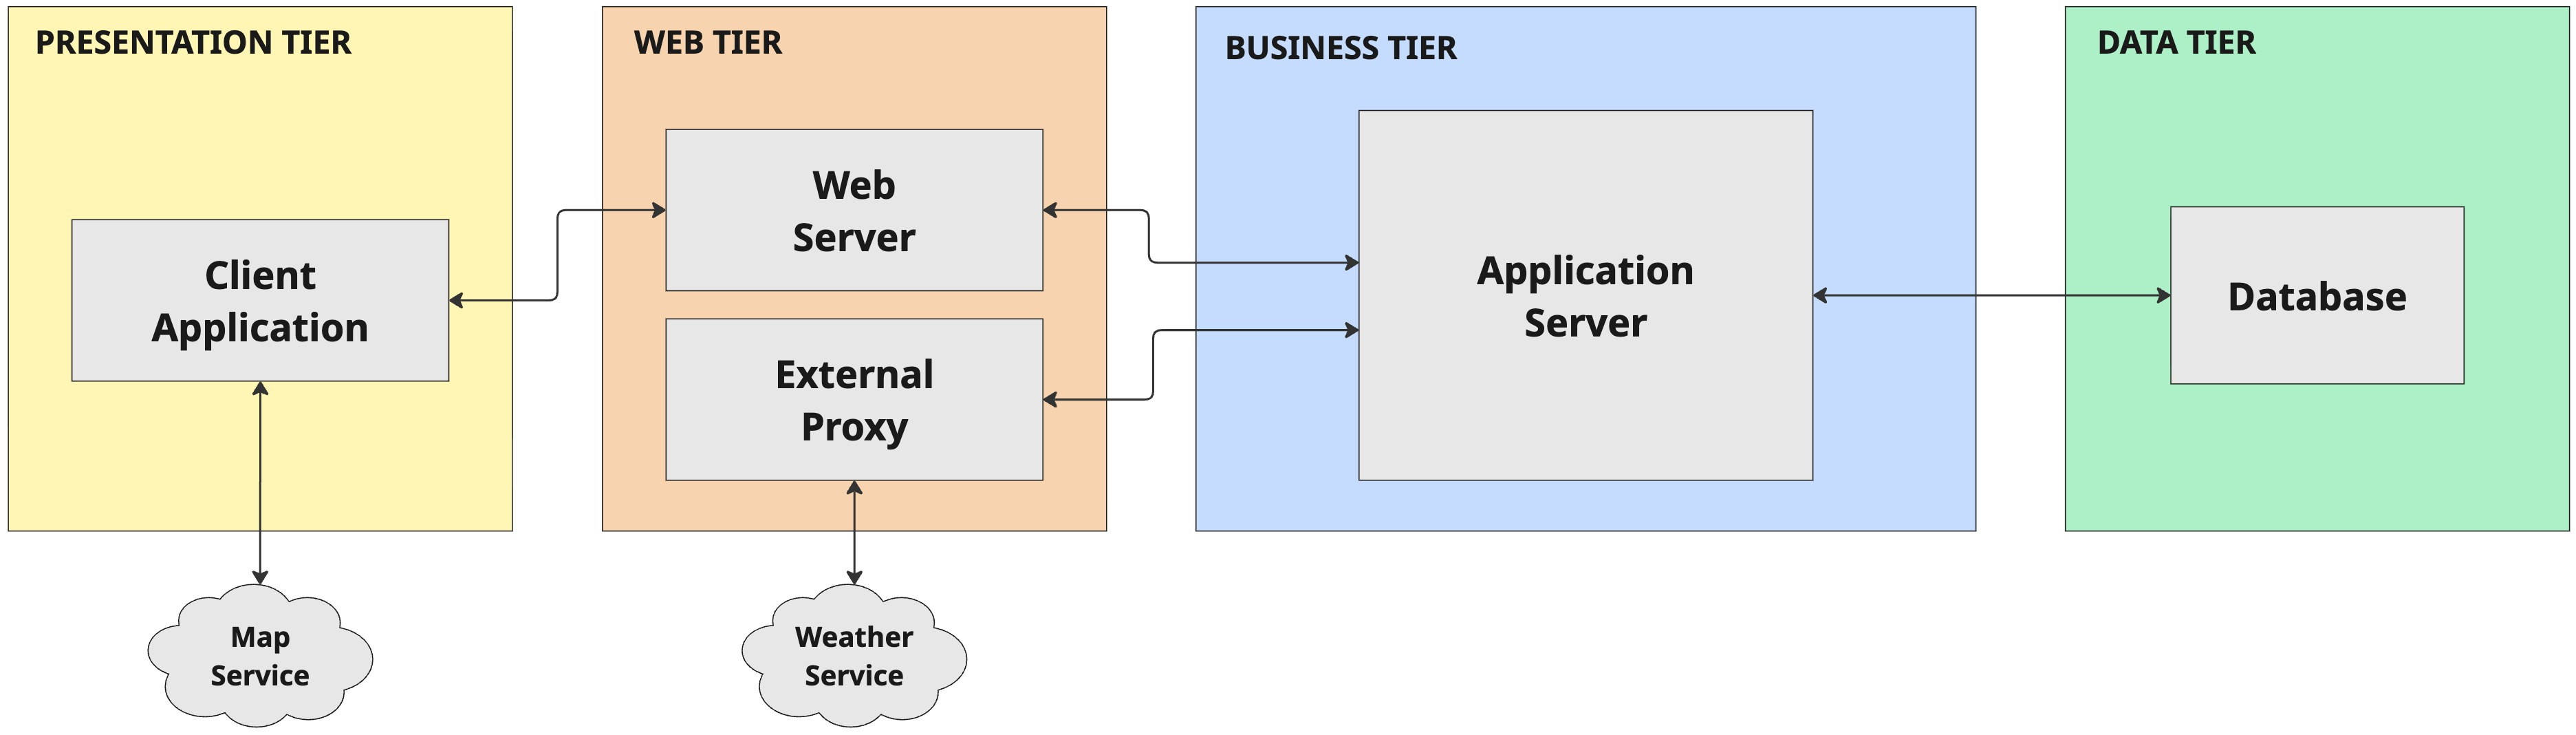
\includegraphics[width=1\linewidth]{DD/Images/4-tier Architecture.jpg}
    \caption{Four-tier architecture}
    \label{fig:placeholder}
\end{figure}

\newpage


\subsubsection{Detailed View}

\textbf{Presentation Tier }\\
The presentation tier of Best Bike Paths (BBP) consists entirely of the interface accessible directly through the user’s device. This layer is responsible for managing human–computer interaction, transforming the cyclist’s actions such as viewing a map or analyzing a path into asynchronous requests to the web tier, and to extract data from the sensors and send them, through the web tier, to the application tier. It also interact with the map service to get the map and the graphical libraries to draw on it.

\vspace{0.3cm}
\noindent
\textbf{Web Tier}\\
The web tier serves as the primary coordination and security layer, and represents the demilitarized zone (DMZ) of the system. It hosts a web server that acts as a reverse proxy, receiving incoming requests from the presentation tier and routing them to the business tier. It also integrates a load balancer to optimize and distribute traffic efficiently across the system. Additionally, this layer includes an external proxy to handle outgoing interactions with the weather service, keeping the business tier isolated from the public network. This centralized approach enables efficient load balancing and ensures that all traffic is strictly monitored and secured before reaching the platform’s internal components.

\vspace{0.3cm}
\noindent
\textbf{Business Tier}\\
The business tier constitutes the logical core of the system, where all the main functionalities of the Best Bike Paths platform are processed. It integrates a load balancer to manage the data distribution across the replicas. Operating within an isolated network, it communicates with the data tier for information persistence through queries. Thanks to its replicated and containerized structure, the tier ensures high scalability and resilience in handling computational workloads.

\vspace{0.3cm}
\noindent
\textbf{Data Tier}\\
The data tier is dedicated to the long-term persistence of all system information, managed through DBMS. It resides in a private network completely isolated from the outside, being accessible exclusively by the business tier to ensure maximum protection of sensitive data. Its replicated structure guarantees the integrity of the information and high availability of the service.

\newpage
\subsection{Component View}
This section presents the Component View of the Best Bike Paths system. It describes the main software components composing each architectural layer and their responsibilities, along with the interfaces through which they interact. The description follows a top-down approach, starting from the most general components and progressively refining the analysis by focusing on the most relevant and complex ones. WeatherServiceI and MapServiceI represent the interfaces of the external services required for the correct functioning of the system


\begin{figure}[!h]
    \centering
    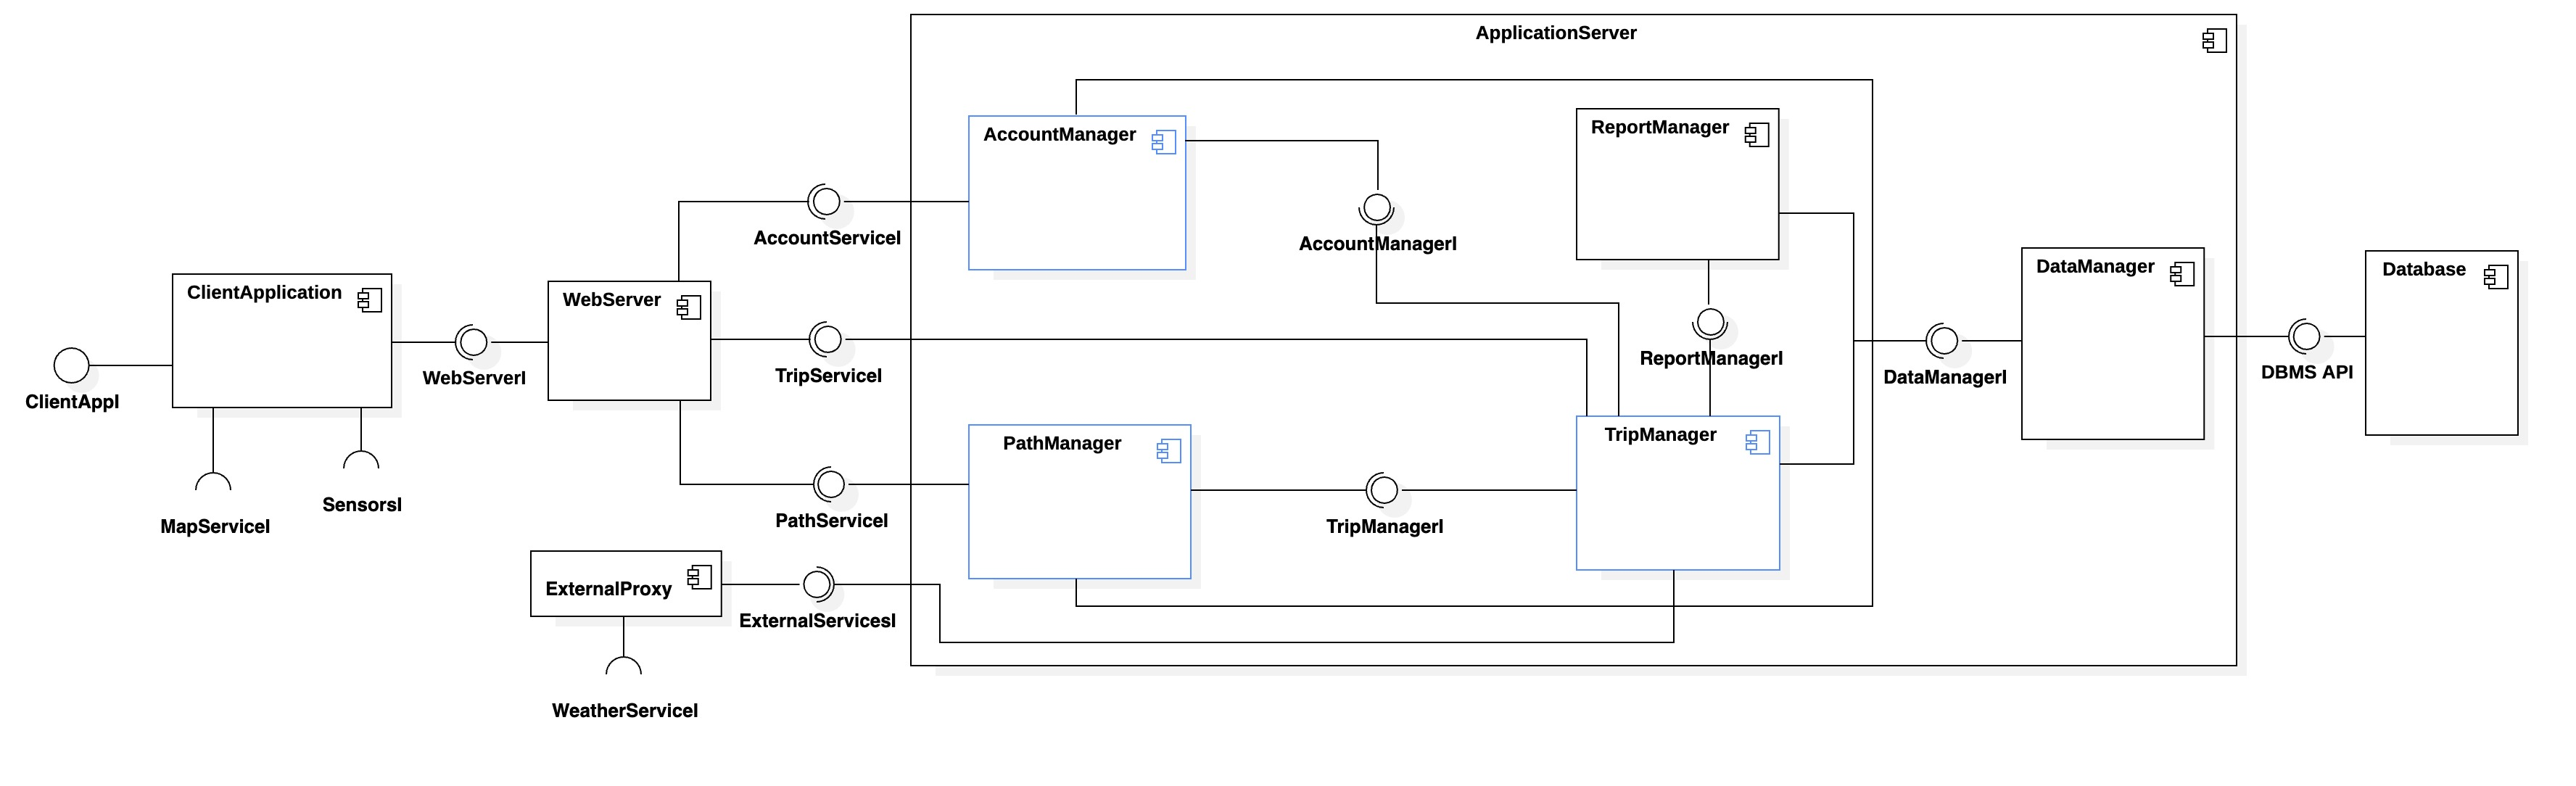
\includegraphics[width=1\linewidth]{DD/Images/Component Diagrams/ComponentDiagram}
    \caption{Component Diagram}
    \label{fig:placeholder}
\end{figure}

\subsubsection{ClientApplication Component}
The ClientApplication Component serves as the Presentation Tier of the application. Its primary function is to render the graphical interfaces enabling end-users to interact with the system's features and services. The component's internal logic is primarily dedicated to interface management, such as preliminary data validation and real-time user feedback. This component is designed for on-road use, providing a portable interface optimized for the cycling experience. It integrates with device hardware to support real-time trip tracking and path-surface monitoring. It offers the complete set of system features in a format that is easy to interact with while on the move, ensuring cyclists have access to all tools during their journeys.


\subsubsection{WebServer Component}
The WebServer component acts as the primary entry point for all incoming traffic from the Presentation Tier. Located within the Web Tier, it handles the reception of HTTPS requests and the logical routing of requests toward the appropriate components of the Business Tier. To ensure scalability and high availability, the Web Server is deployed in multiple replicated instances behind a load balancer. Incoming requests are distributed among these replicas, allowing the system to handle higher traffic volumes and to remain operational in case of individual instance failures.

\newpage
\subsubsection{ExternalProxy component}
The ExternalProxy, located within the Web Tier, is the component dedicated to the centralized management of all outgoing (outbound) communications to third-party service providers. It acts as an intermediary between the Business Tier and external APIs of weather service, required to enrich path information. This separation ensures that the Business Tier remains isolated from the public network, delegating to the proxy the task of interacting with the external world in a secure and controlled manner.

\subsubsection{ApplicationServer Component}
The ApplicationServer, located in the Business Tier, is responsible for executing the entire application logic, processing validated requests coming from the Web Tier. Operating within an isolated private network, it communicates with the Data Tier for information persistence and with the ExternalProxy for retrieving weather data, ensuring high scalability and resilience through a replicated and containerized structure. It is divided into the following components:

\begin{itemize}
    \item \textbf{AccountManager}\vspace{0.3mm}\\
    The Account Manager component handles all operations related to user identity, security, and profile evolution. It exposes the \textit{AccountServiceI} interface for external interactions and the \textit{AccountManagerI} interface to provide user-related data to other internal components. It communicates with the Data Manager through the \textit{DataManagerI} interface to ensure the persistence and integrity of user credentials and statistics.

    \begin{figure}[!h]
        \centering
        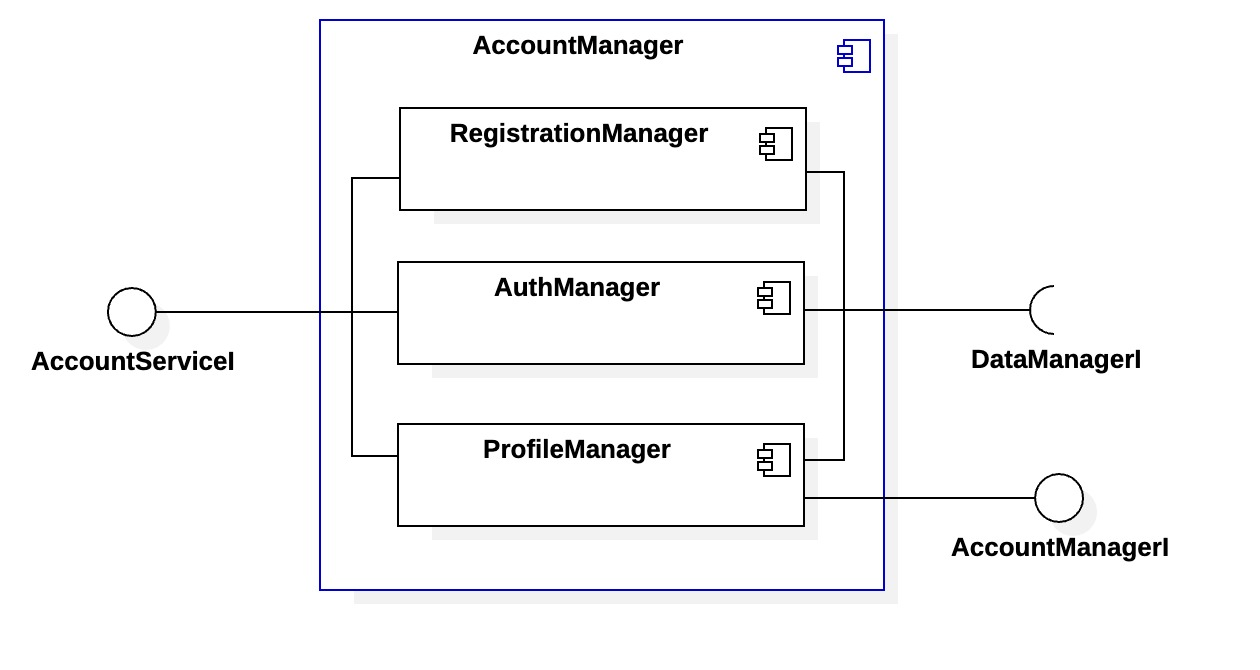
\includegraphics[width=0.7\linewidth]{DD/Images/Component Diagrams/AccountManager.jpg}
        \caption{Account Manager}
        \label{fig:placeholder}
    \end{figure}
    \begin{enumerate}
        \item \textbf{RegistrationManager} \vspace{0.3mm} \\
        It manages the cyclists registration. It is responsible for validating user input, ensuring the uniqueness of emails, and initializing basic performance statistics. It interacts with the \textit{DataManagerI} to store new profile records.
        \item \textbf{AuthManager} \vspace{0.3mm} \\ 
        Represents the core of system security. It manages session tokens, password encryption, and access permissions, ensuring that every sensitive operation is strictly authorized.
        \item \textbf{ProfileManager} \vspace{0.3mm} \\
        Administers the cyclist's profile and handles the modification of personal data. It tracks cumulative performance metrics, specifically the total distance traveled and global average speed, interfacing with the persistence layer to provide an up-to-date summary of the user's activity.
    \end{enumerate}
    \item \textbf{PathManager}\vspace{0.3mm}\\
    The Path Manager handles path's lifecycle. It provides the \textit{PathServiceI} to allow the WebServer to send request from the ClientApplication. It relies on the \textit{DataManagerI} for path data and the \textit{TripManagerI} to save a trip.

    \begin{figure}[!h]
        \centering
        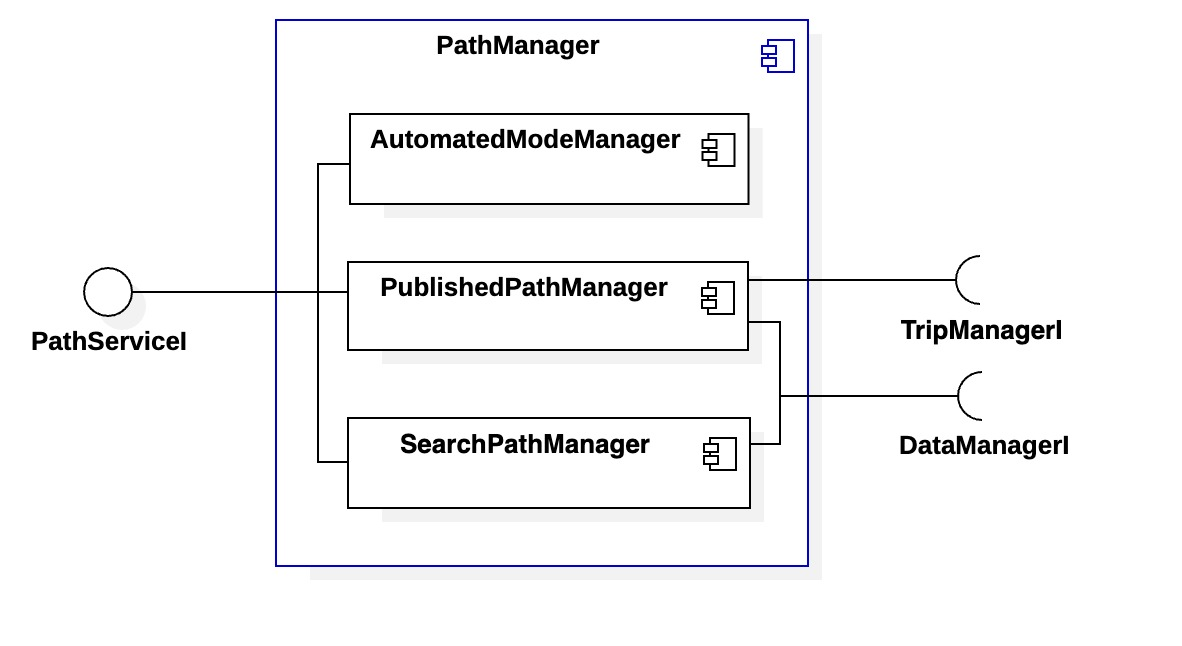
\includegraphics[width=0.8\linewidth]{DD/Images/Component Diagrams/PathManager.jpg}
        \caption{Path Manager}
        \label{fig:placeholder}
    \end{figure}

    \begin{enumerate}
        \item \textbf{AutomatedModeManager} \vspace{0.3mm} \\
        Manages the passive tracking logic. When a user begins a trip without a pre-set destination, this sub-component analyzes movements and reconstructs the path in real-time.
        \item \textbf{PublishedPathManager} \vspace{0.3mm} \\
        It handles path management and the manual mode.
        \item \textbf{SearchPathManager} \vspace{0.3mm} \\
        Provides the filtering engines. It allows the path database to be queried by provinding origin and destination of path of interest, and returns .
    \end{enumerate}
    \newpage
    \item \textbf{TripManager}\vspace{0.3mm}\\
    The Trip Manager provides the \textit{TripServiceI} to allow users to visualize the trip history and manage the trip navigation, and the \textit{TripManagerI} interface to manage the trip history. It requests services from the Account Manager (\textit{AccountManagerI}) to make account's data consistent, from the Report Manager (\textit{ReportManagerI}) to report obstacle and status updates, and from the Data Manager (\textit{DataManagerI}) for history storage. It uses \textit{ExternalServicesI} to access weather services.
    \begin{figure}[!h]
        \centering
        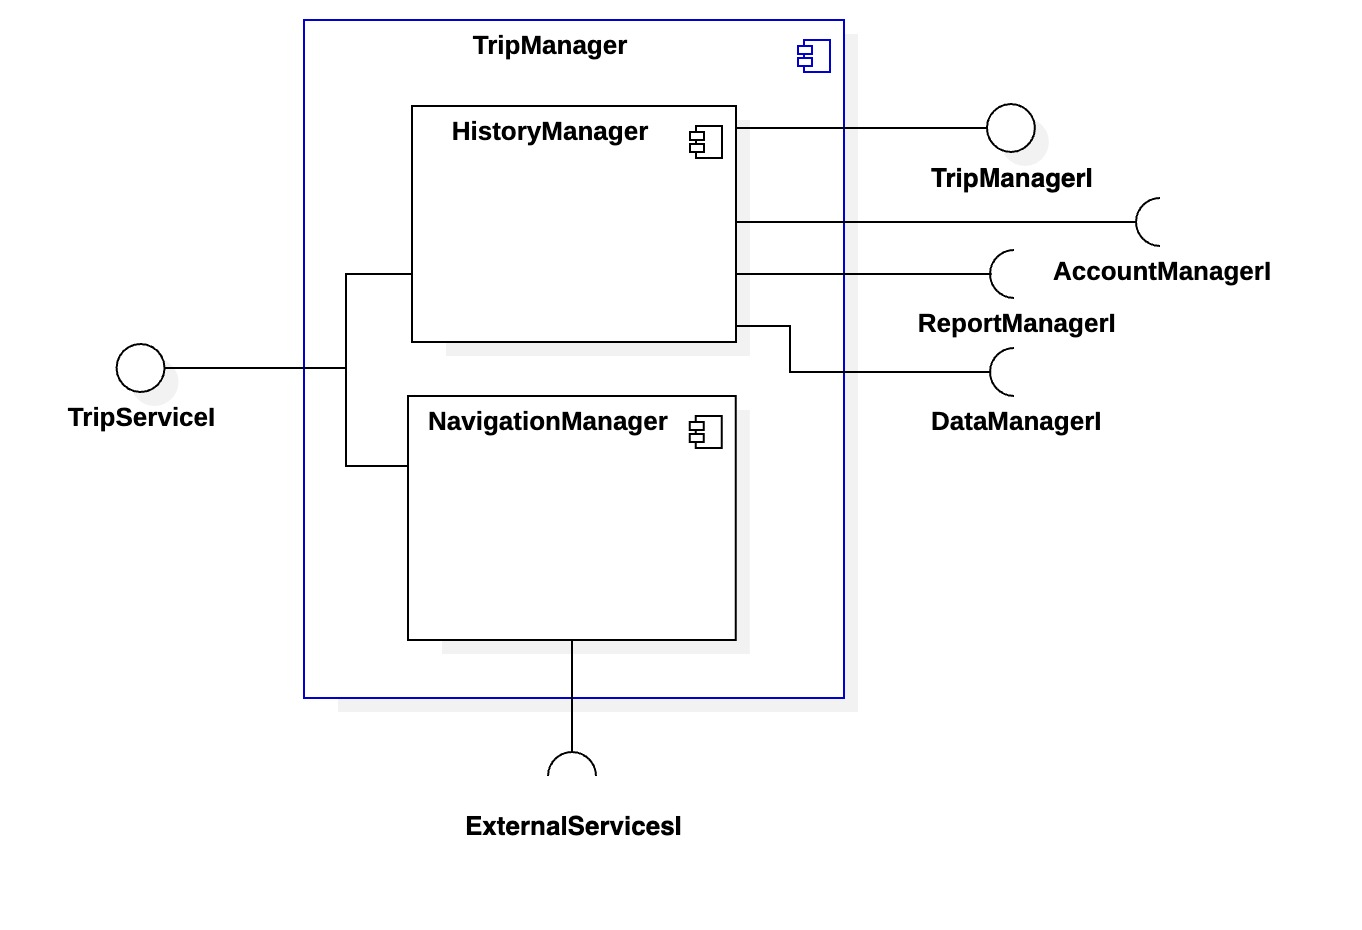
\includegraphics[width=0.8\linewidth]{DD/Images/Component Diagrams/TripManager.jpg}
        \caption{Trip Manager}
        \label{fig:placeholder}
    \end{figure}
    \begin{enumerate}
        \item \textbf{NavigationManager}\\
        Processes GPS data to provide guidance instructions and
        compares the current location against the planned path.
        \item \textbf{HistoryManager}\\
        Once a session is finalized, it consolidates all trip data including average speed and total distance. It then invokes the \textit{DataManagerI} to archive the trip for later viewing on the dashboard.
    \end{enumerate}
    \item \textbf{ReportManager}\vspace{0.3mm}\\
    The Report Manager exposes the \textit{ReportManagerI} interface to receive real-time alerts and status updates from the Trip Manager and uses the \textit{DataManagerI} to store all reported information. This component collects reports originating from navigations, whose information can be modified manually at the end of the naviagation. Reports concerning the same path, collected within the same timeframe, are merged to update path status and obstacle detection within the PathManager. This establishes a virtuous cycle where every user contributes to collective safety.
\end{itemize}

\newpage
\subsubsection{Data Component}

The Database is an external component dedicated to the secure and permanent storage of all system information.

\begin{itemize}
    \item \textbf{Role}: It serves as the central repository for sensitive user profiles, the library of published bike paths, historical trips, and reported path obstacles and status.
    
    \item \textbf{Interaction}: It communicates exclusively with the DataManager via the DBMS API interface. This separation ensures data integrity and optimized CRUD operations.
    
\end{itemize}

\subsubsection{External Services}
\begin{itemize}
    \item \textbf{Map Service}\vspace{0.3mm}\\
    Provides the foundational geographic data. It offers detailed road network information, enabling the system to visualize paths and guide users.
    \item \textbf{Weather Service}\vspace{0.3mm}\\
    Delivers real-time atmospheric telemetry, including temperature, wind speed, and current conditions.
\end{itemize}

\subsection{Deployment View}
The Deployment View describes the physical mapping of software components onto hardware nodes and the network infrastructure, illustrating the system’s distribution and defining its container organization. The following figure shows the platform’s deployment diagram.


\begin{figure}[!h]
    \centering
    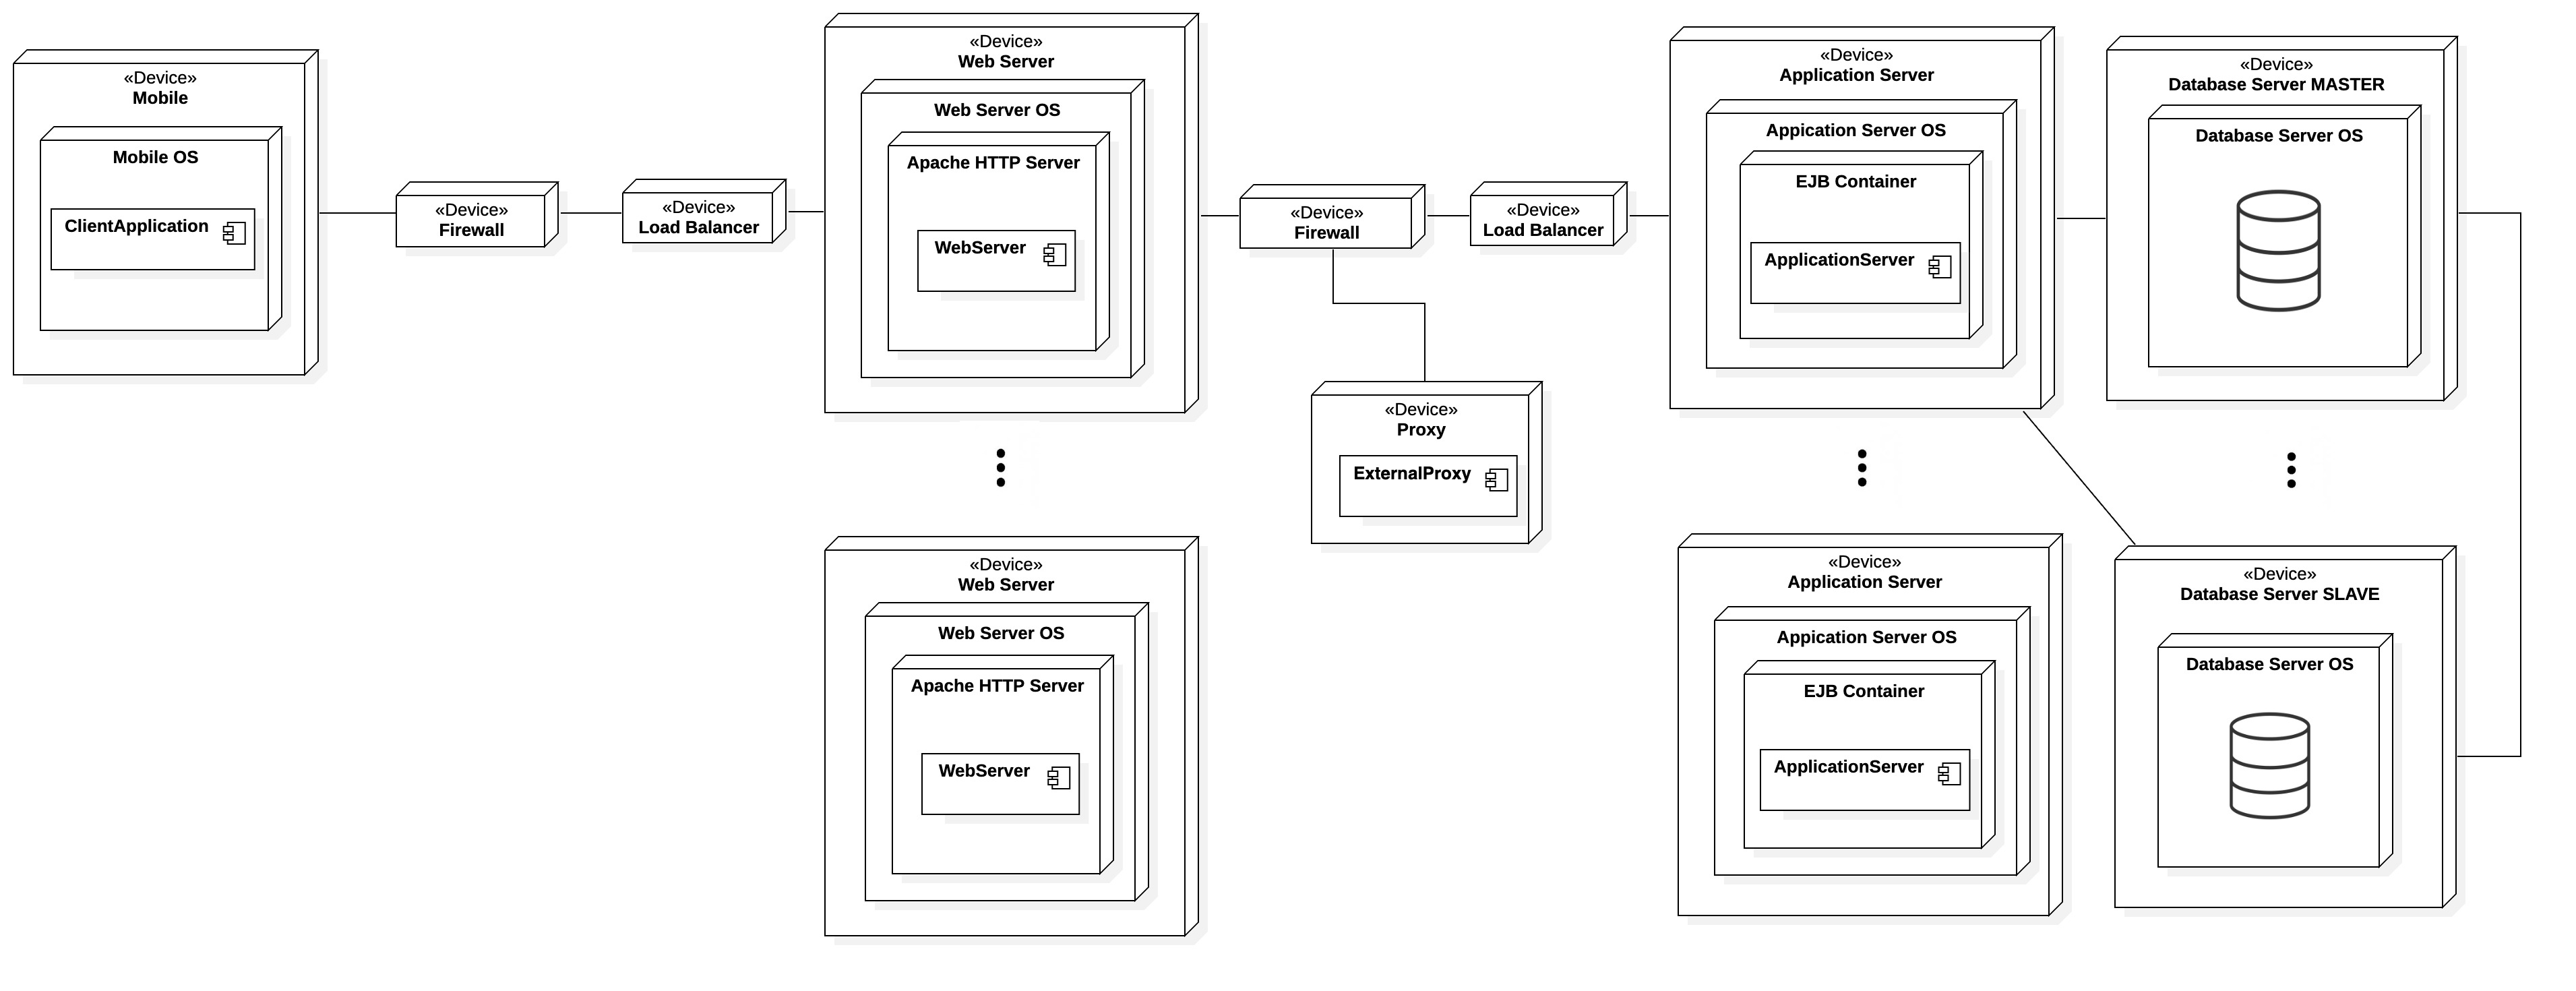
\includegraphics[width=1\linewidth]{DD/Images/DeploymentDiagram}
    \caption{Deployment Diagram}
    \label{fig:placeholder}
\end{figure}

\noindent
This Deployment View illustrates a four-layer architecture designed to ensure scalability and security through a clear separation of responsibilities. Incoming traffic from the presentation tier first passes through a firewall and is then distributed by an initial load balancer among multiple replicas of the web server, optimizing request handling and service availability. Similarly, calls to the business logic pass through another firewall and are then handled by a second load balancer, which distributes the load across the ApplicationServer replicas.
The data tier adopts a master–slave architecture in which the ApplicationServer and its replicas read from and write to the master, which continuously updates the slaves. In the case of a master failure, the ApplicationServer and its replicas read data from the slaves. Outbound calls to weather service pass through the proxy, preventing the direct exposure of the application server’s IP address. In this case, the responses received from the weather service pass through the firewall which, unlike the data flow coming from the web server, forwards them directly to the application server without passing through the load balancer.

\subsection{Runtime View}
This section describes the dynamic behavior of the system during its execution, illustrating how components interact with each other to fulfill the functional requirements. Unlike static views, this section focuses on control flows, message exchanges, and the sequencing of operations among the various components defined in the component view. Through the analysis of the use cases defined in the RASD document, it enables a clear understanding of the request lifecycle and the coordination of processes in real time.

\vspace{3mm}
\noindent
\textbf{[SD1] Signup Sequence Diagram}
\begin{figure}[!h]
    \centering
    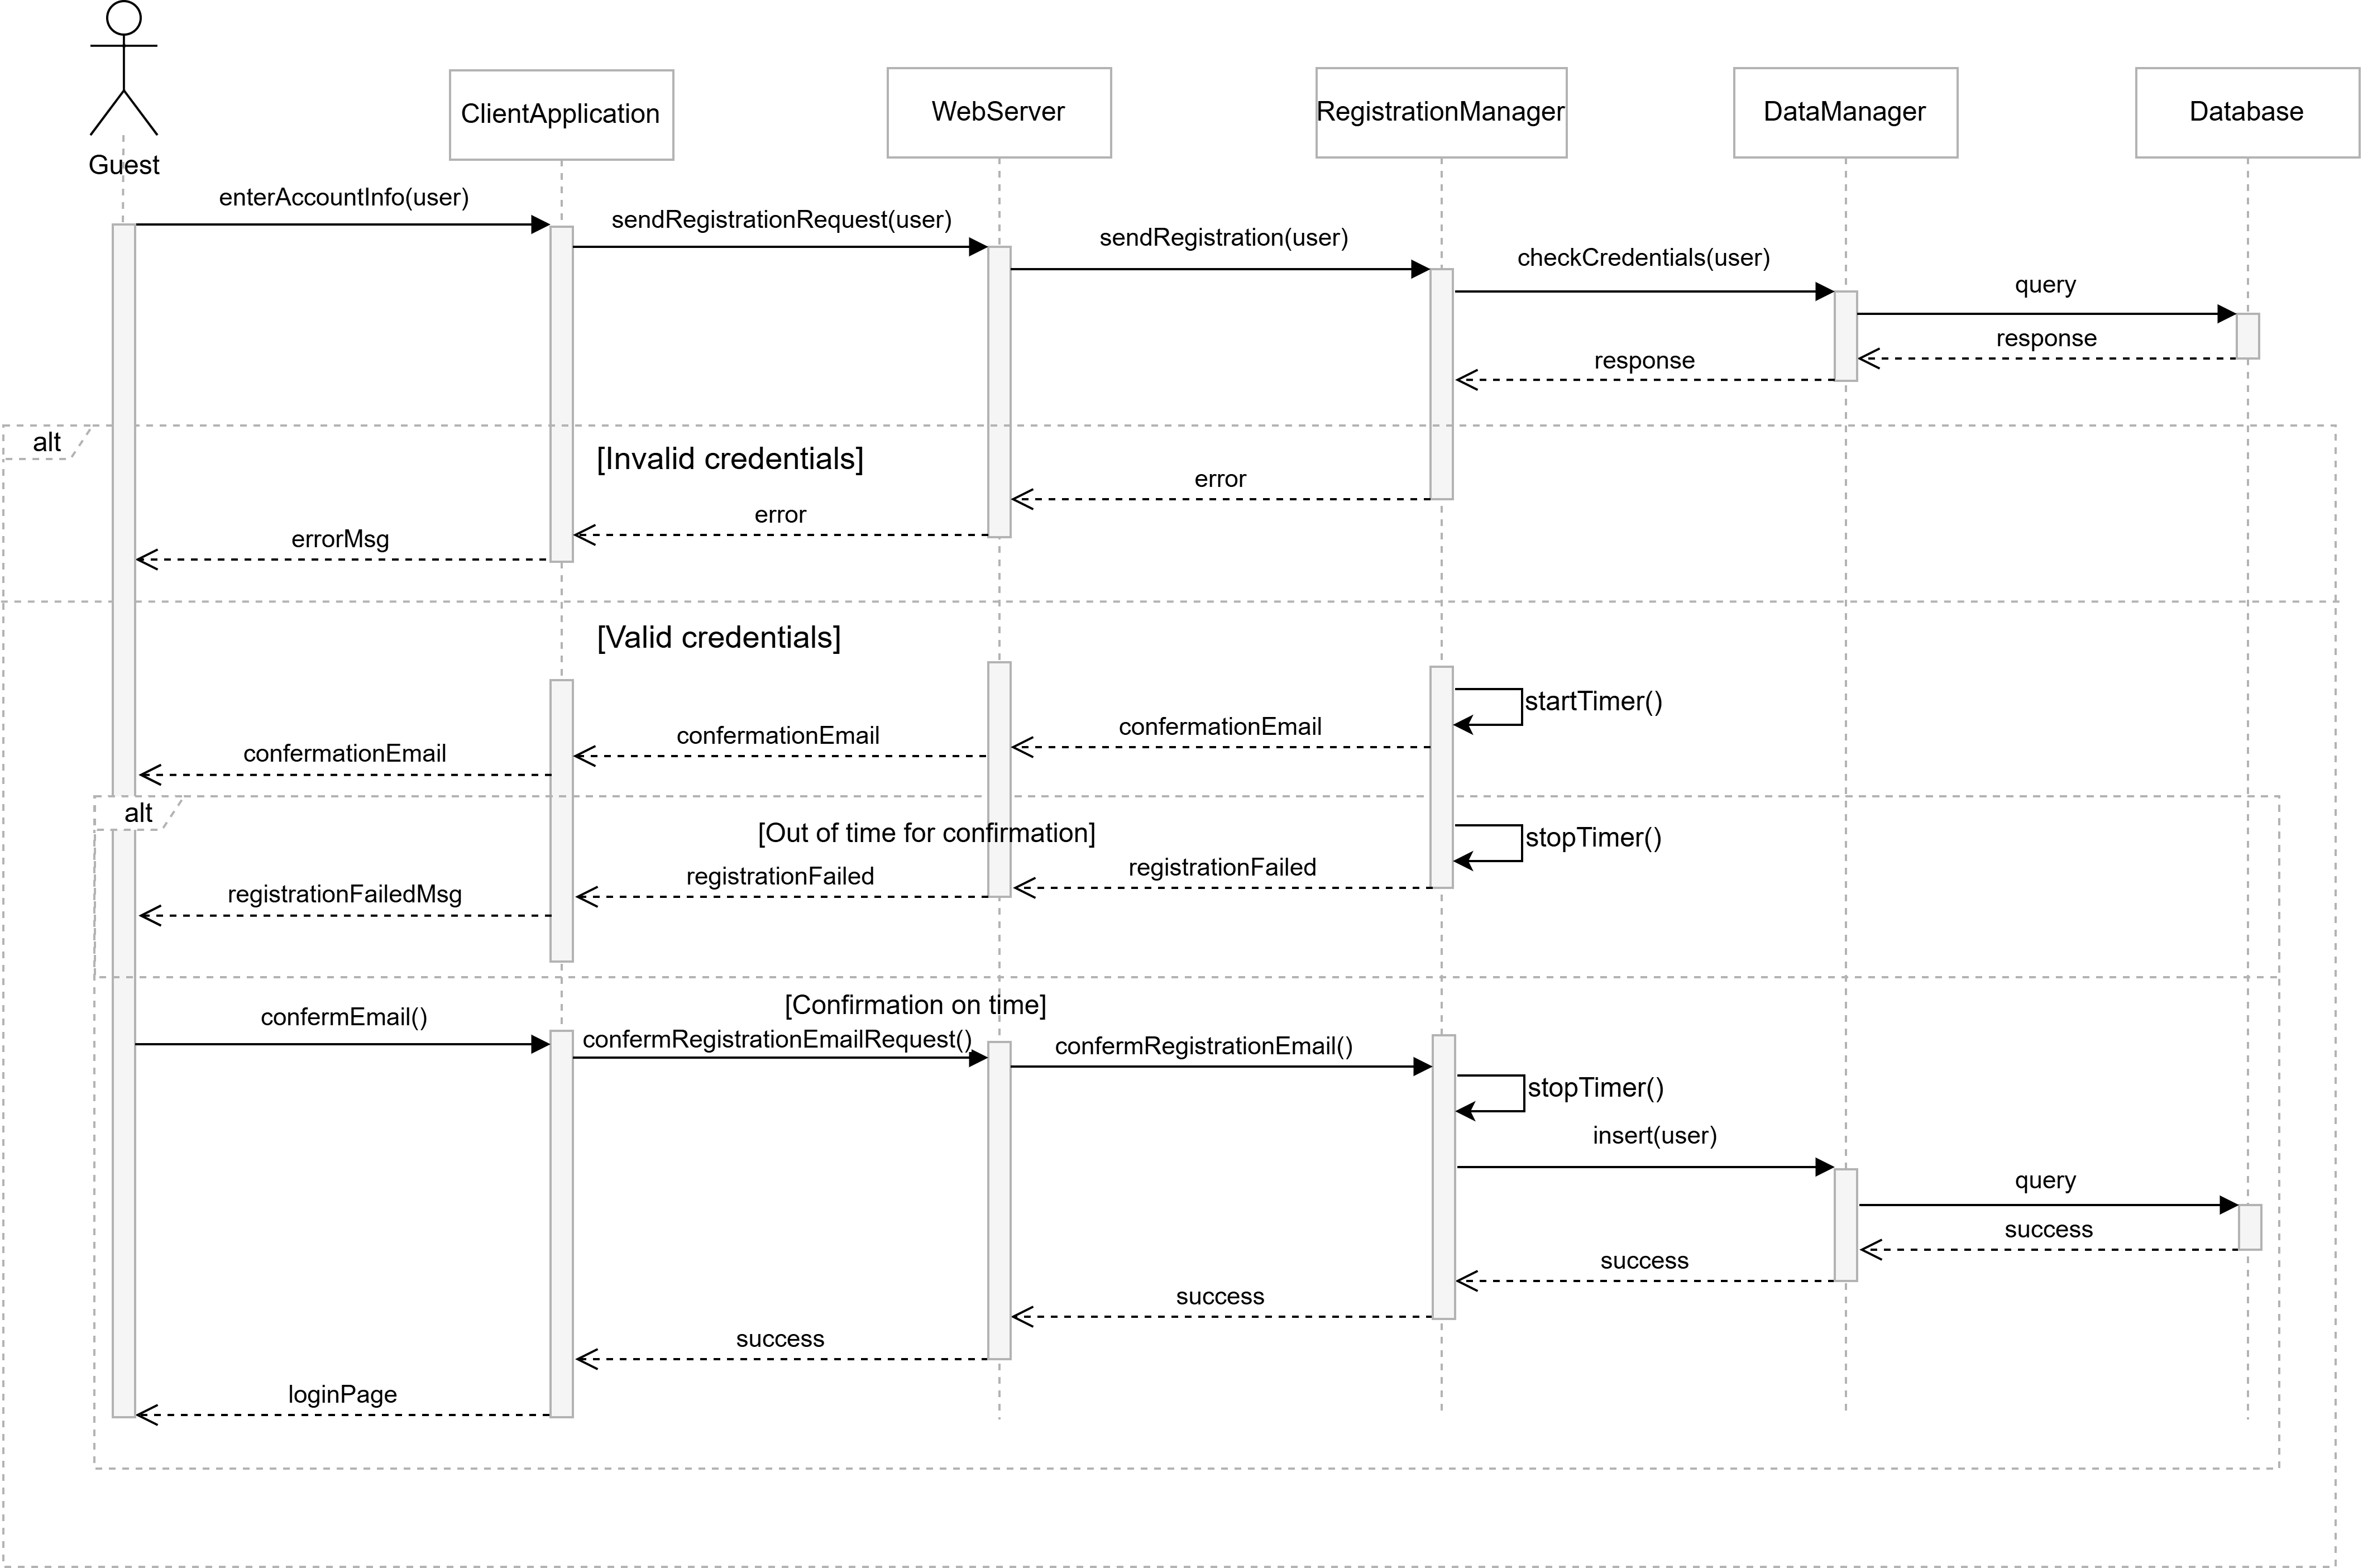
\includegraphics[width=1\linewidth]{DD/Images/SequenceDiagram/Signup.png}
    \caption{[SD1] Signup Sequence Diagram}
    \label{fig:placeholder}
\end{figure}
\\
This sequence diagram describes the registration flow. The RegistrationManager first validates the submitted credentials; if valid, it initiates a time-bound verification process by sending a confirmation email and starting an internal timer.

The process has two possible outcomes based on user action:
\begin{itemize}
    \item The operation aborts if the initial credentials are invalid or if the user fails to confirm the email before the timer expires.
    \item The system permanently inserts the new user into the Database only if the Guest confirms the registration within the validity window.
\end{itemize}
\newpage
\noindent
\textbf{[SD2] Login Sequence Diagram}
\begin{figure}[!h]
    \centering
    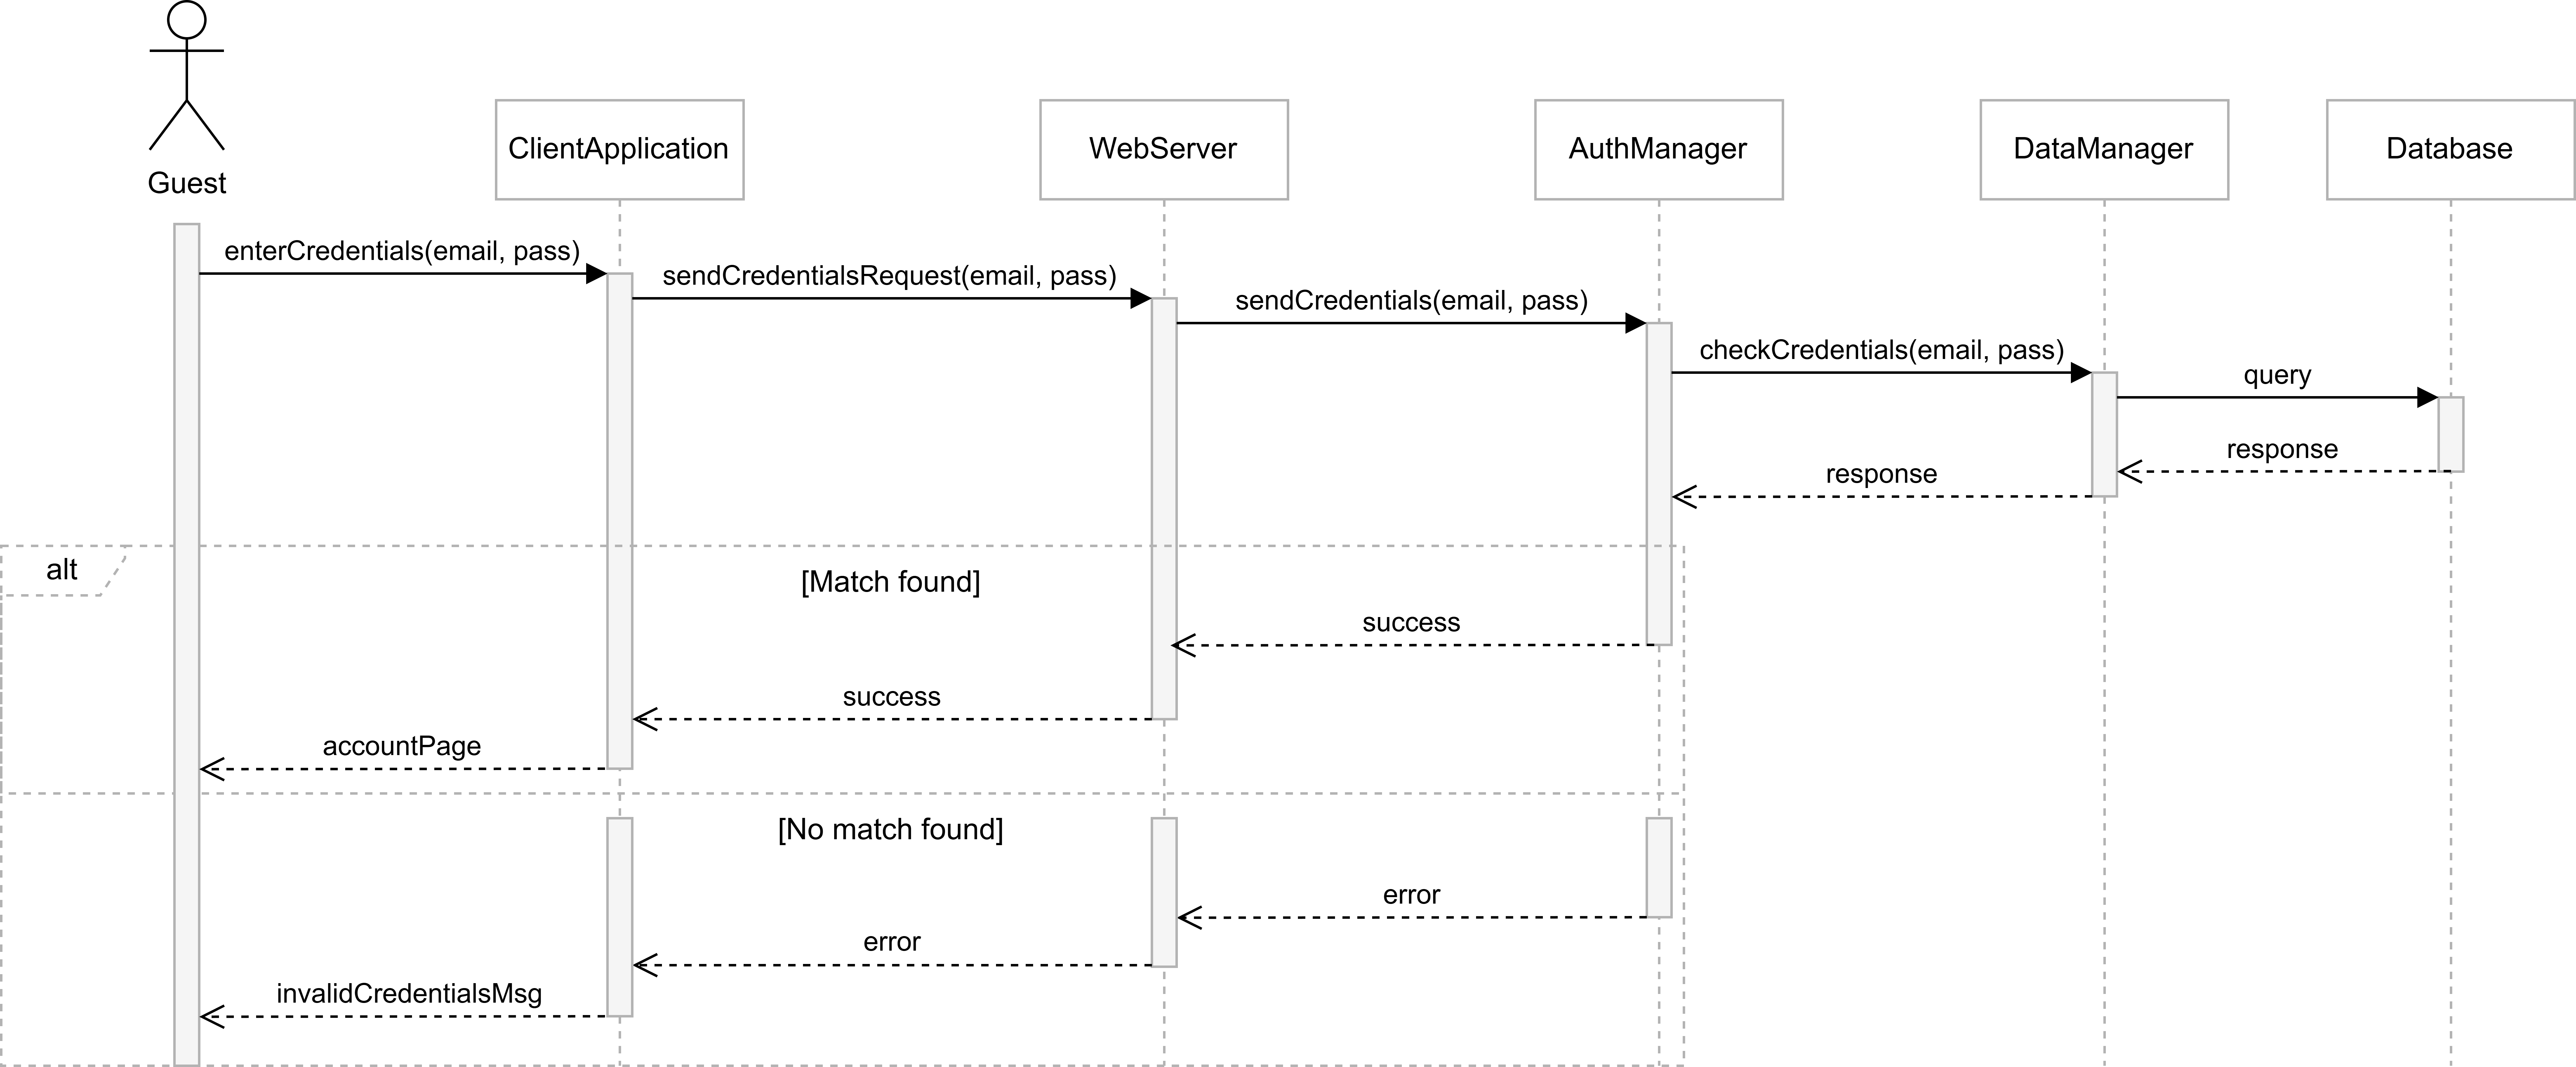
\includegraphics[width=1\linewidth]{DD/Images/SequenceDiagram/Login.png}
    \caption{[SD2] Login Sequence Diagram}
    \label{fig:placeholder}
\end{figure}
\\
This sequence diagram describes the login process of a guest. The guest enters their email and password in the ClientApplication, which forwards the credentials to the WebServer. The WebServer passes them to the AuthManager, which asks the DataManager to verify the credentials by querying the Database.
\begin{itemize}
    \item If the credentials match (match found), the successful result propagates back through the chain and the guest is redirected to the account page.
    \item If no match is found, an error is returned and the ClientApplication displays an invalidCredentials message to the guest trip.
\end{itemize}

\newpage
\noindent
\textbf{[SD3] Search Path Sequence Diagram}

\begin{figure}[H]
    \centering
    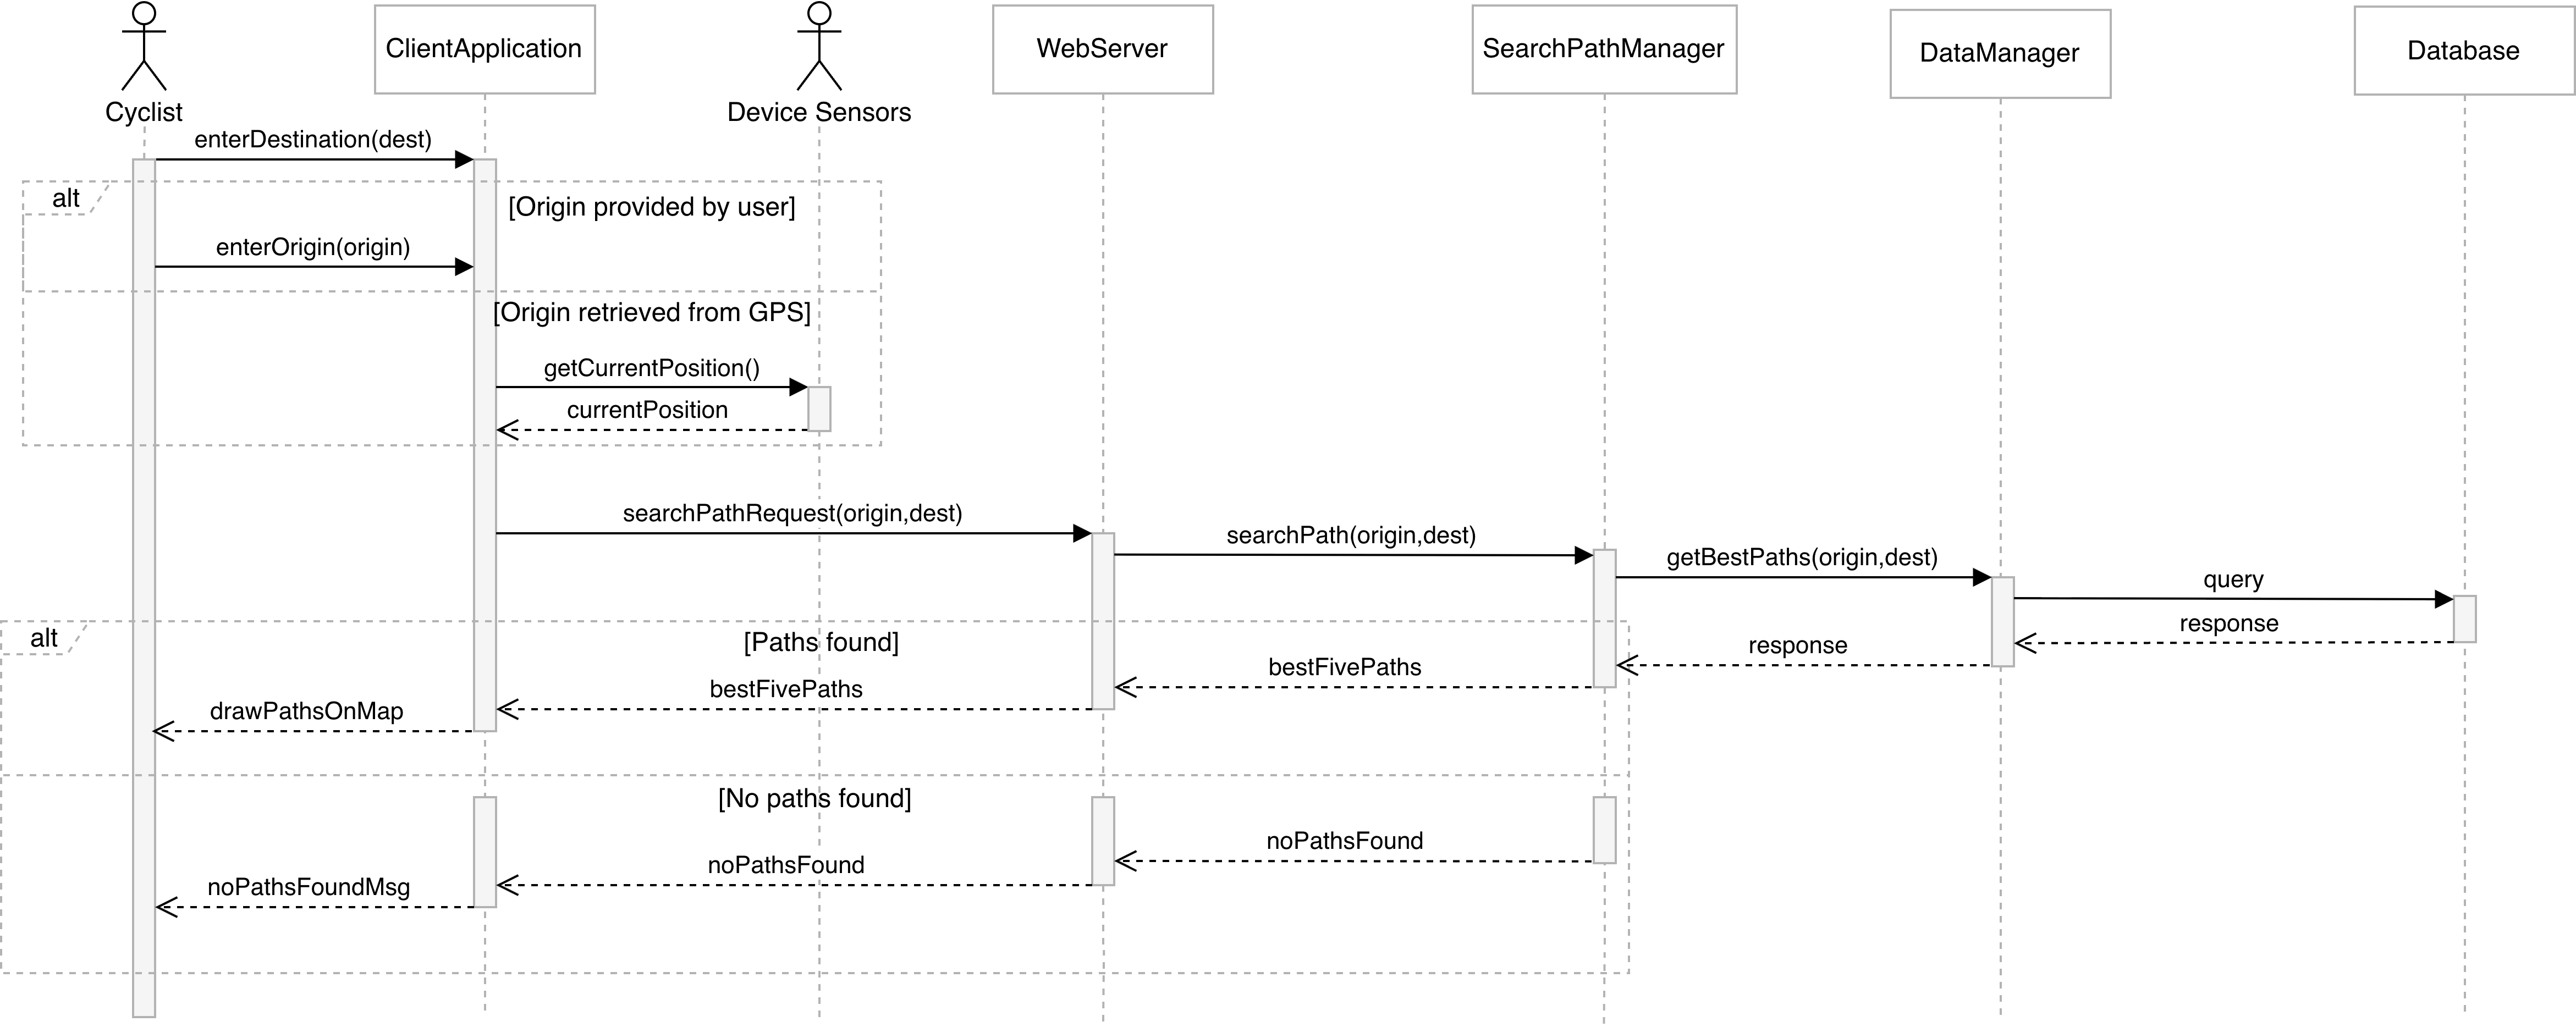
\includegraphics[width=1\linewidth]{DD//Images//SequenceDiagram/SearchPath.png}
    \caption{[SD3] Search Path Sequence Diagram}
    \label{fig:placeholder}
\end{figure}

\noindent
This sequence diagram describes the path search process initiated by a cyclist. It is assumed that, upon opening the application, the cyclist is on the home page and the map has already been loaded by the SearchPathManager through the MapService. The interaction begins with the Cyclist entering the destination in the ClientApplication. An alternative flow determines the origin: it is either manually provided by the user (enterOrigin) or automatically retrieved from the Device Sensors via the GPS (getCurrentPosition). Once the origin and destination are established, the ClientApplication sends a request to the WebServer. The WebServer forwards the request to the SearchPathManager, which is responsible for the search logic. The SearchPathManager then contacts the DataManager, which interacts with the Database to query for the best paths.

\begin{itemize}
    \item If paths are found, the bestFivePaths data is propagated back through the system (via the SearchPathManager and WebServer) to the ClientApplication, which then performs the drawPathsOnMap action to visualize the paths for the cyclist.
    \item Otherwise, if no suitable paths are found, a noPathsFound signal is returned through the layers, and a specific message (noPathsFoundMsg) is displayed to inform the cyclist.
\end{itemize}

\newpage
\noindent
\textbf{[SD4] Start Navigation Sequence Diagram}
\begin{figure}[!h]
    \centering
    \includegraphics[width=1\linewidth]{DD/Images/SequenceDiagram/StartNavigation.png}
    \caption{[SD4] Start Navigation Sequence Diagram}
    \label{fig:placeholder}
\end{figure}
\\
This sequence diagram describes the assisted navigation process for a cyclist, from the start until the completion of the trip. The Cyclist starts the navigation from the ClientApplication, which sends a start request to the WebServer. The NavigationManager initializes the navigation, starts a timer, and signals that the system is ready; the client then displays the navigation page. During the trip (loop block, until the destination is reached), the application retrieves the current position from the device sensors, updates the cursor on the map, displays the current road via the Map Service, and sends requests to the server to compute metrics based on the path and the current position.
The NavigationManager checks whether the cyclist remains on the path and computes navigation metrics.
\begin{itemize}
    \item If the cyclist stays on the path, the current speed is sent to the client and displayed to the user.
    \item If the cyclist deviates from the path for too long, a deviation is reported, the timer is stopped, and the navigation is terminated.
\end{itemize}
At the end of the trip, he client requests the weather from the weather service and the path geometry from the Map Service. The NavigationManager, through the ExternalProxy, queries the Weather Service, processes the result (the most frequent weather condition along the path), and sends it to the client, which displays the trip completion page with the final information.

\newpage
\noindent
\textbf{[SD5] Save Trip Sequence Diagram}
\begin{figure}[!h]
    \centering
    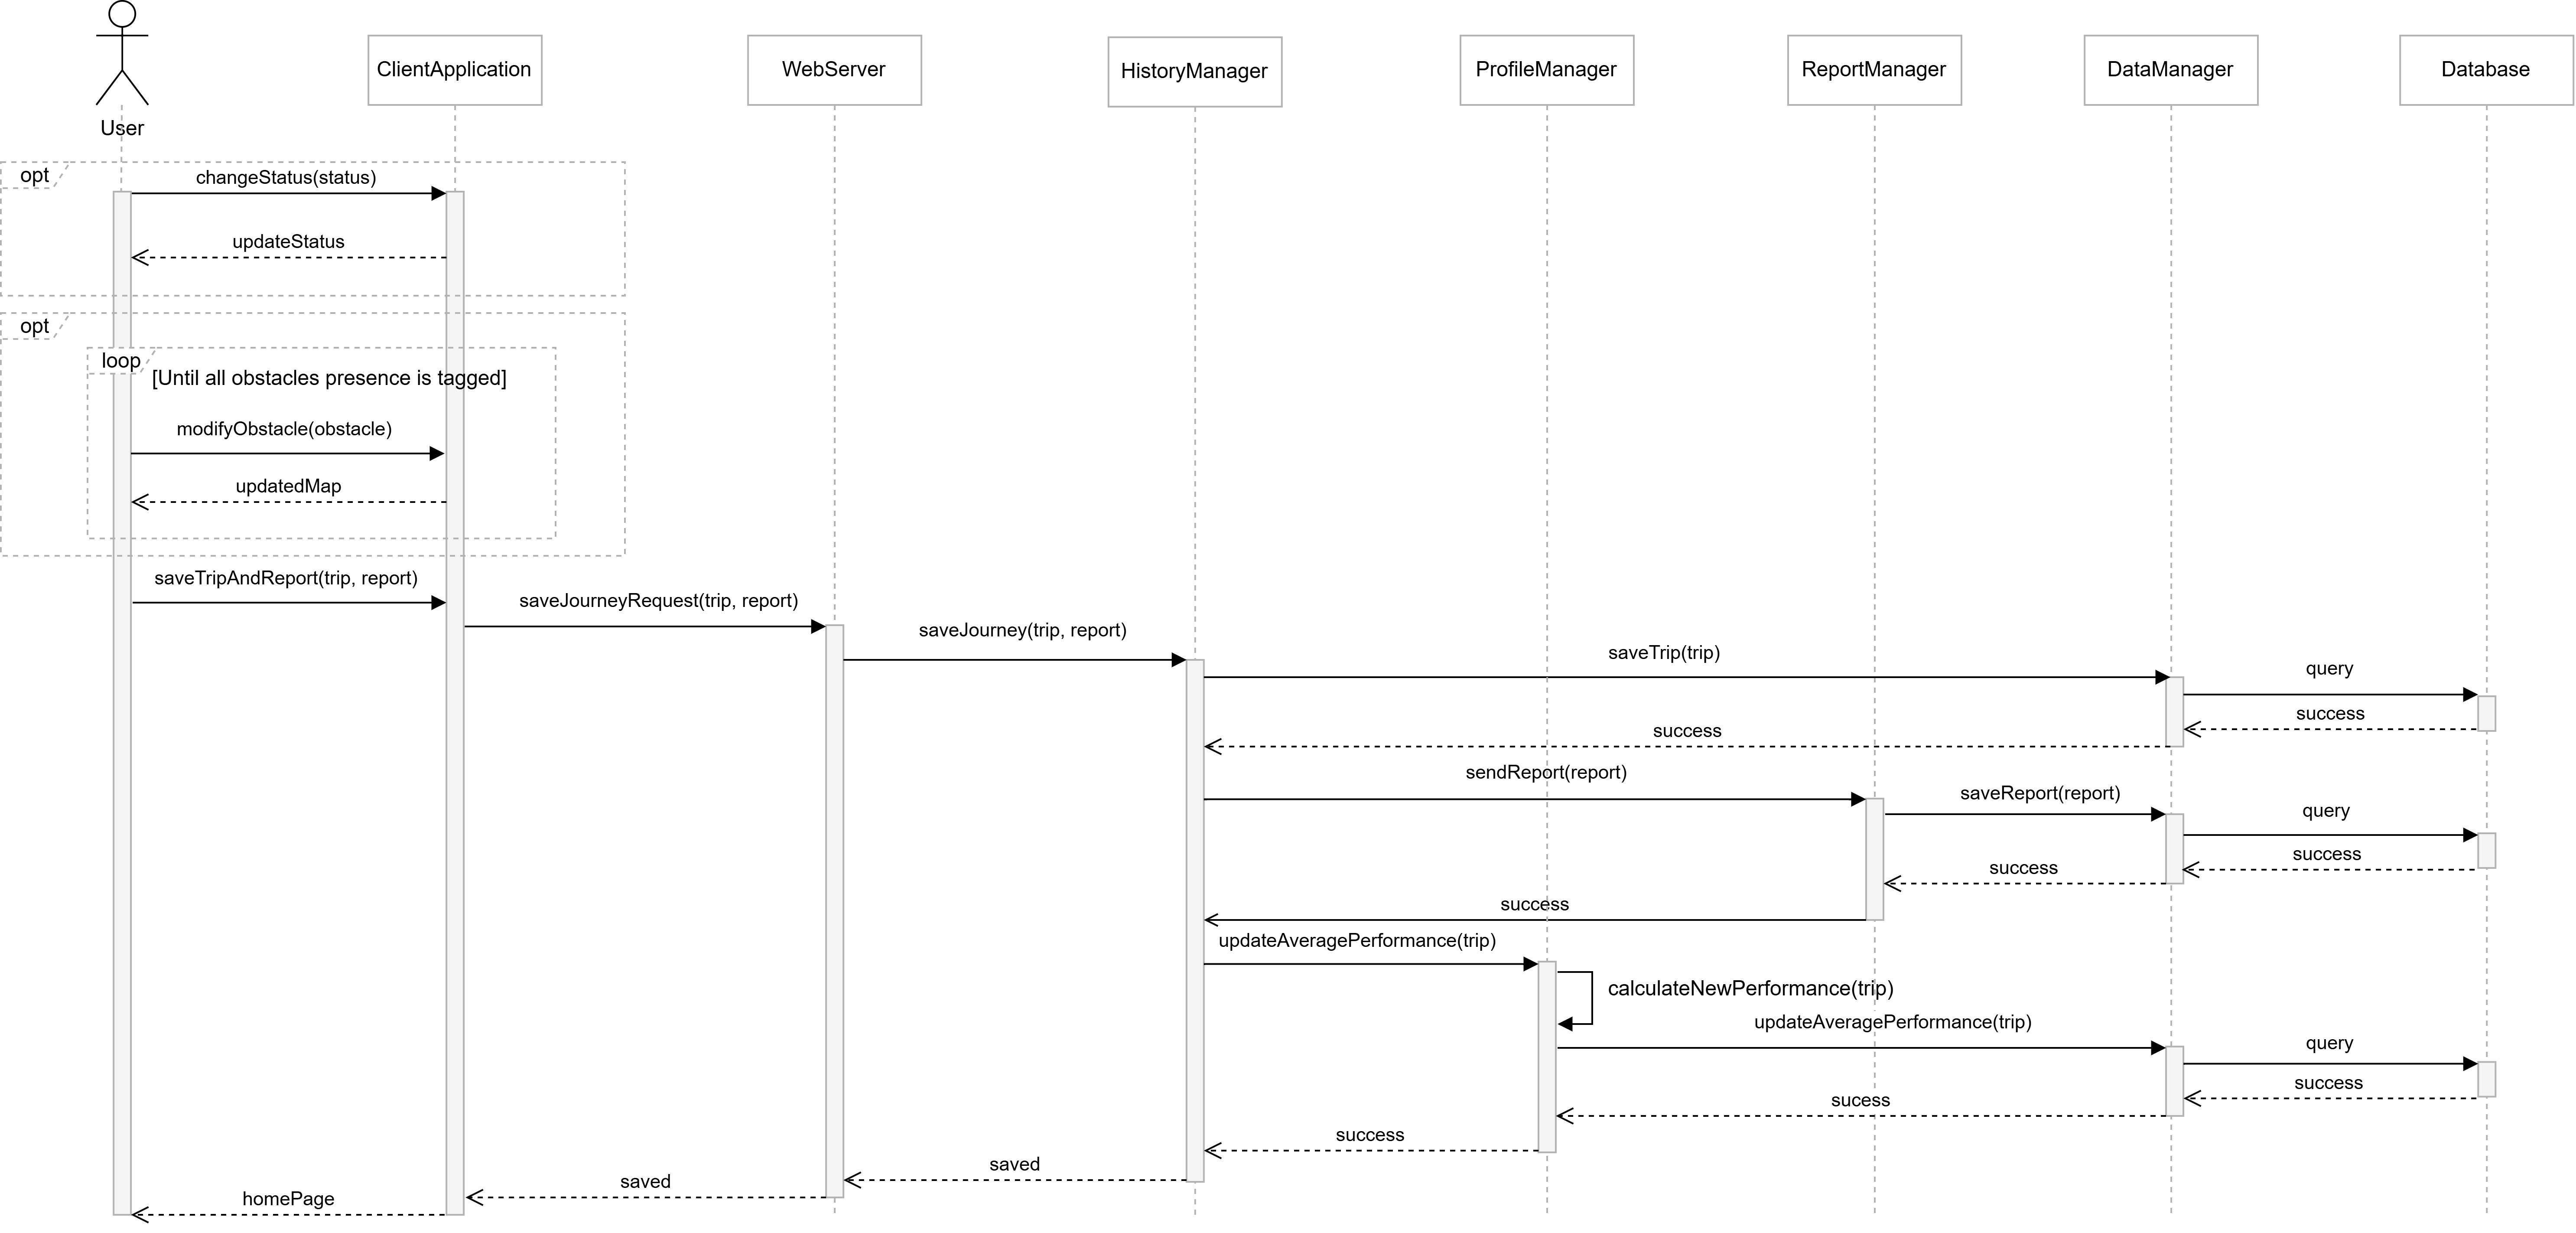
\includegraphics[width=1\linewidth]{DD/Images/SequenceDiagram/SaveTrip.png}
    \caption{[SD5] Save Trip Sequence Diagram}
    \label{fig:placeholder}
\end{figure}
\\
This sequence diagram illustrates the Save Trip workflow. The process could initiate with the user changes path status via the interface. An optional sequence, structured as a loop, allows the user to iteratively modify obstacle presence directly on the interface. The core persistence phase is triggered when the user saves the trip and report. The WebServer forwards this combined data to the HistoryManager, which coordinates the operation. First, it directly persists the trip data via the DataManager. Then, it delegates the report details to the ReportManager, which saves the report in the database via the DataManager. Finally, the HistoryManager interacts with the ProfileManager to calculate and update the user's average performance statistics. Upon the successful completion of this chain of operations, the success response propagates back through the system, and the user is redirected to the homepage.

\newpage
\noindent
\textbf{[SD6] View Trips Sequence Diagram}
\begin{figure}[h!]
    \centering
    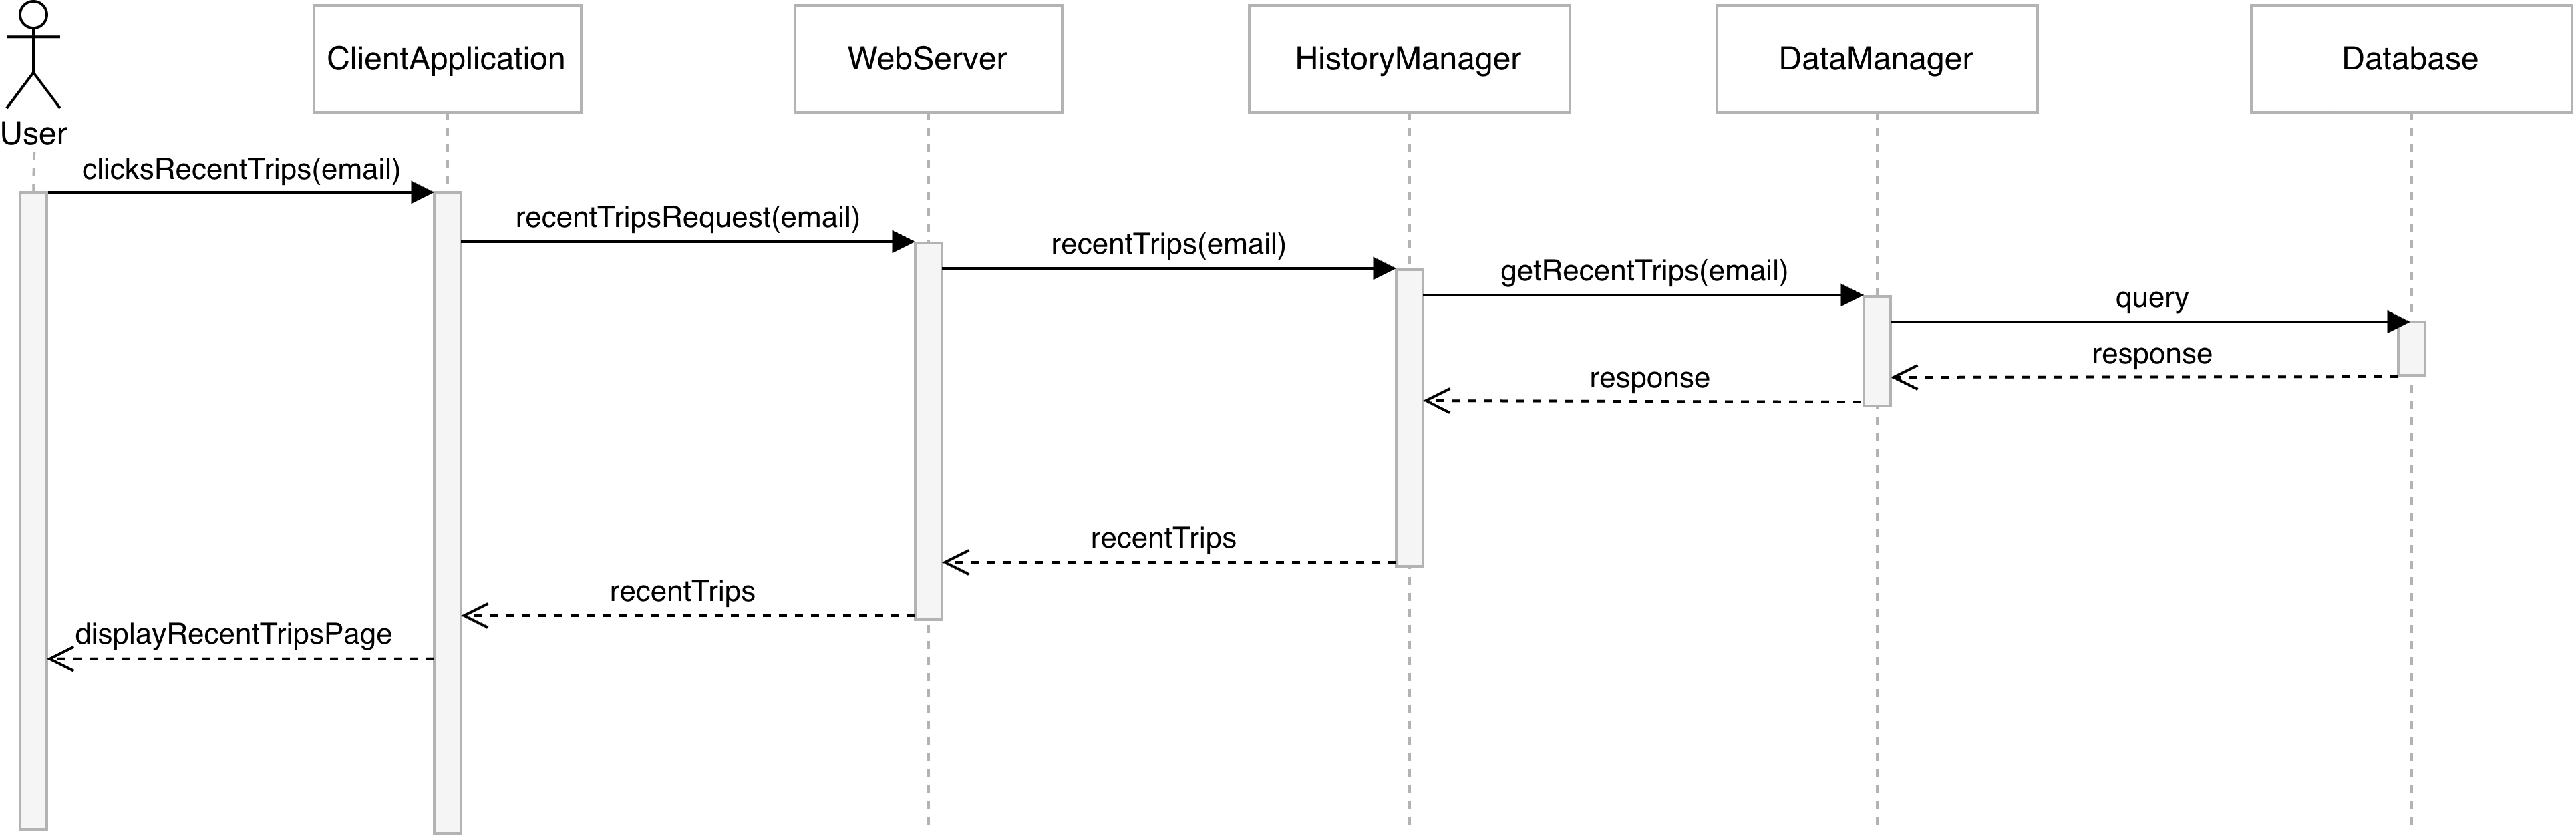
\includegraphics[width=1\linewidth]{DD//Images//SequenceDiagram/ViewTrips.png}
    \caption{[SD6] View Trips Sequence Diagram}
    \label{fig:placeholder}
\end{figure}

\noindent
This sequence diagram shows the process of displaying the trips performed by the user in the dedicated section of the application, called Recent Trips. Initially, the user clicks on the Recent Trips option in the interface. This action triggers the ClientApplication to send a request containing the user identifier to the WebServer. The WebServer then forwards the request to the HistoryManager, which is responsible for handling the retrieval of the user’s travel history. The HistoryManager contacts the DataManager in order to obtain the list of recent trips associated with the given user. The DataManager queries the Database and retrieves the corresponding data. The response is then propagated back from the Database to the DataManager and subsequently to the HistoryManager. Once the HistoryManager has received the list of recent trips, this information is sent back through the WebServer to the ClientApplication. Finally, the ClientApplication displays the Recent Trips page to the user, presenting the retrieved trips in the user interface.




\newpage
\noindent
\textbf{[SD7] Edit Profile Sequence Diagram}
\begin{figure}[!h]
    \centering
    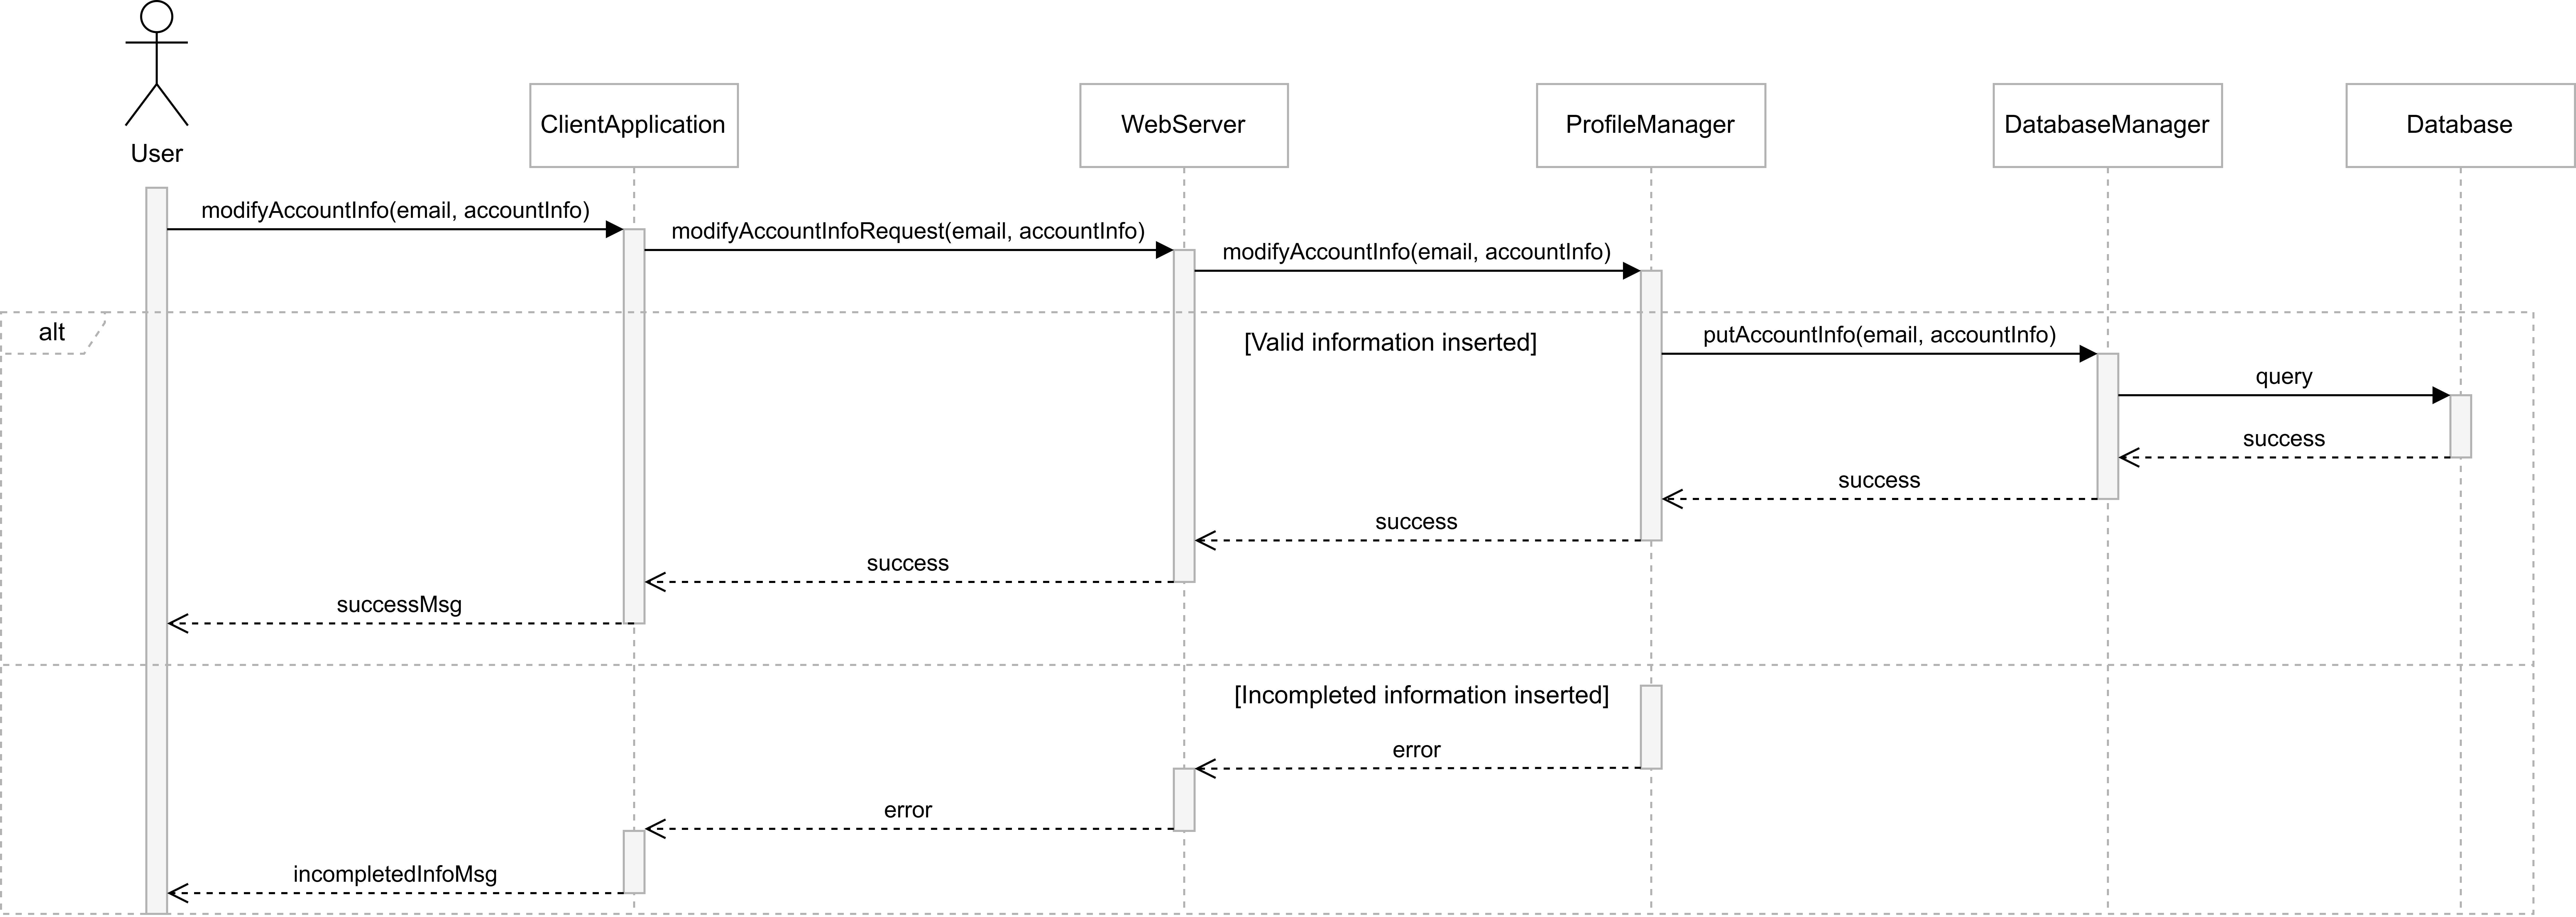
\includegraphics[width=1\linewidth]{DD/Images/SequenceDiagram/EditProfileInfo.png}
    \caption{[SD7] Edit Profile Sequence Diagram}
    \label{fig:placeholder}
\end{figure}
\\
This sequence diagram describes the process of updating user profile information.
The User sends the update request through the ClientApplication, which forwards it to the WebServer and then to the ProfileManager.
The ProfileManager validates the submitted data and, if valid, asks the DatabaseManager to update the information in the Database.
\begin{itemize}
    \item If the information is valid, the update is successfully completed, a success response propagates back through the chain, and the ClientApplication displays a confirmation message to the user.
    \item If the information is incomplete, an error is returned, propagates back to the ClientApplication, and is shown to the user as an incomplete data message.
\end{itemize}

\vspace{15mm}
\noindent
\textbf{[SD8] Delete Path Sequence Diagram}
\begin{figure}[!h]
    \centering
        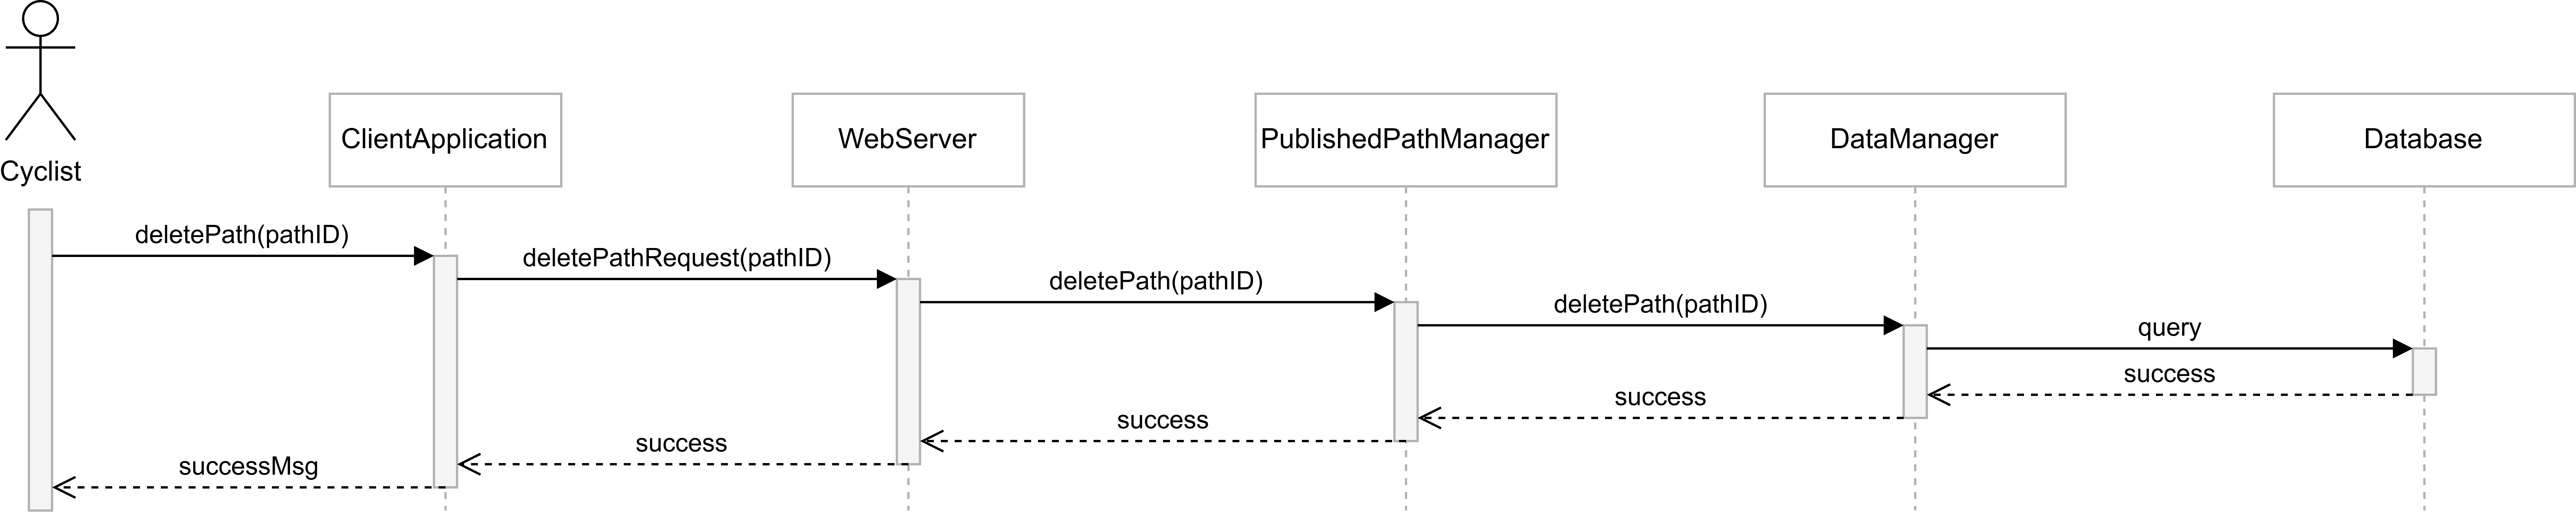
\includegraphics[width=1\linewidth]{DD/Images/SequenceDiagram/DeletePath.png}
    \caption{[SD8] Delete Path Sequence Diagram}
    \label{fig:placeholder}
\end{figure}
\\
This sequence diagram illustrates the process of deleting a path initiated by a cyclist, showing how the request is propagated through the various architectural layers down to the Database. Once the deletion query is executed, the success message propagates back through the entire component chain to confirm the operation to the end user.

\newpage
\noindent
\textbf{[SD9] Publish Path Sequence Diagram}
\begin{figure} [h!]
    \centering
    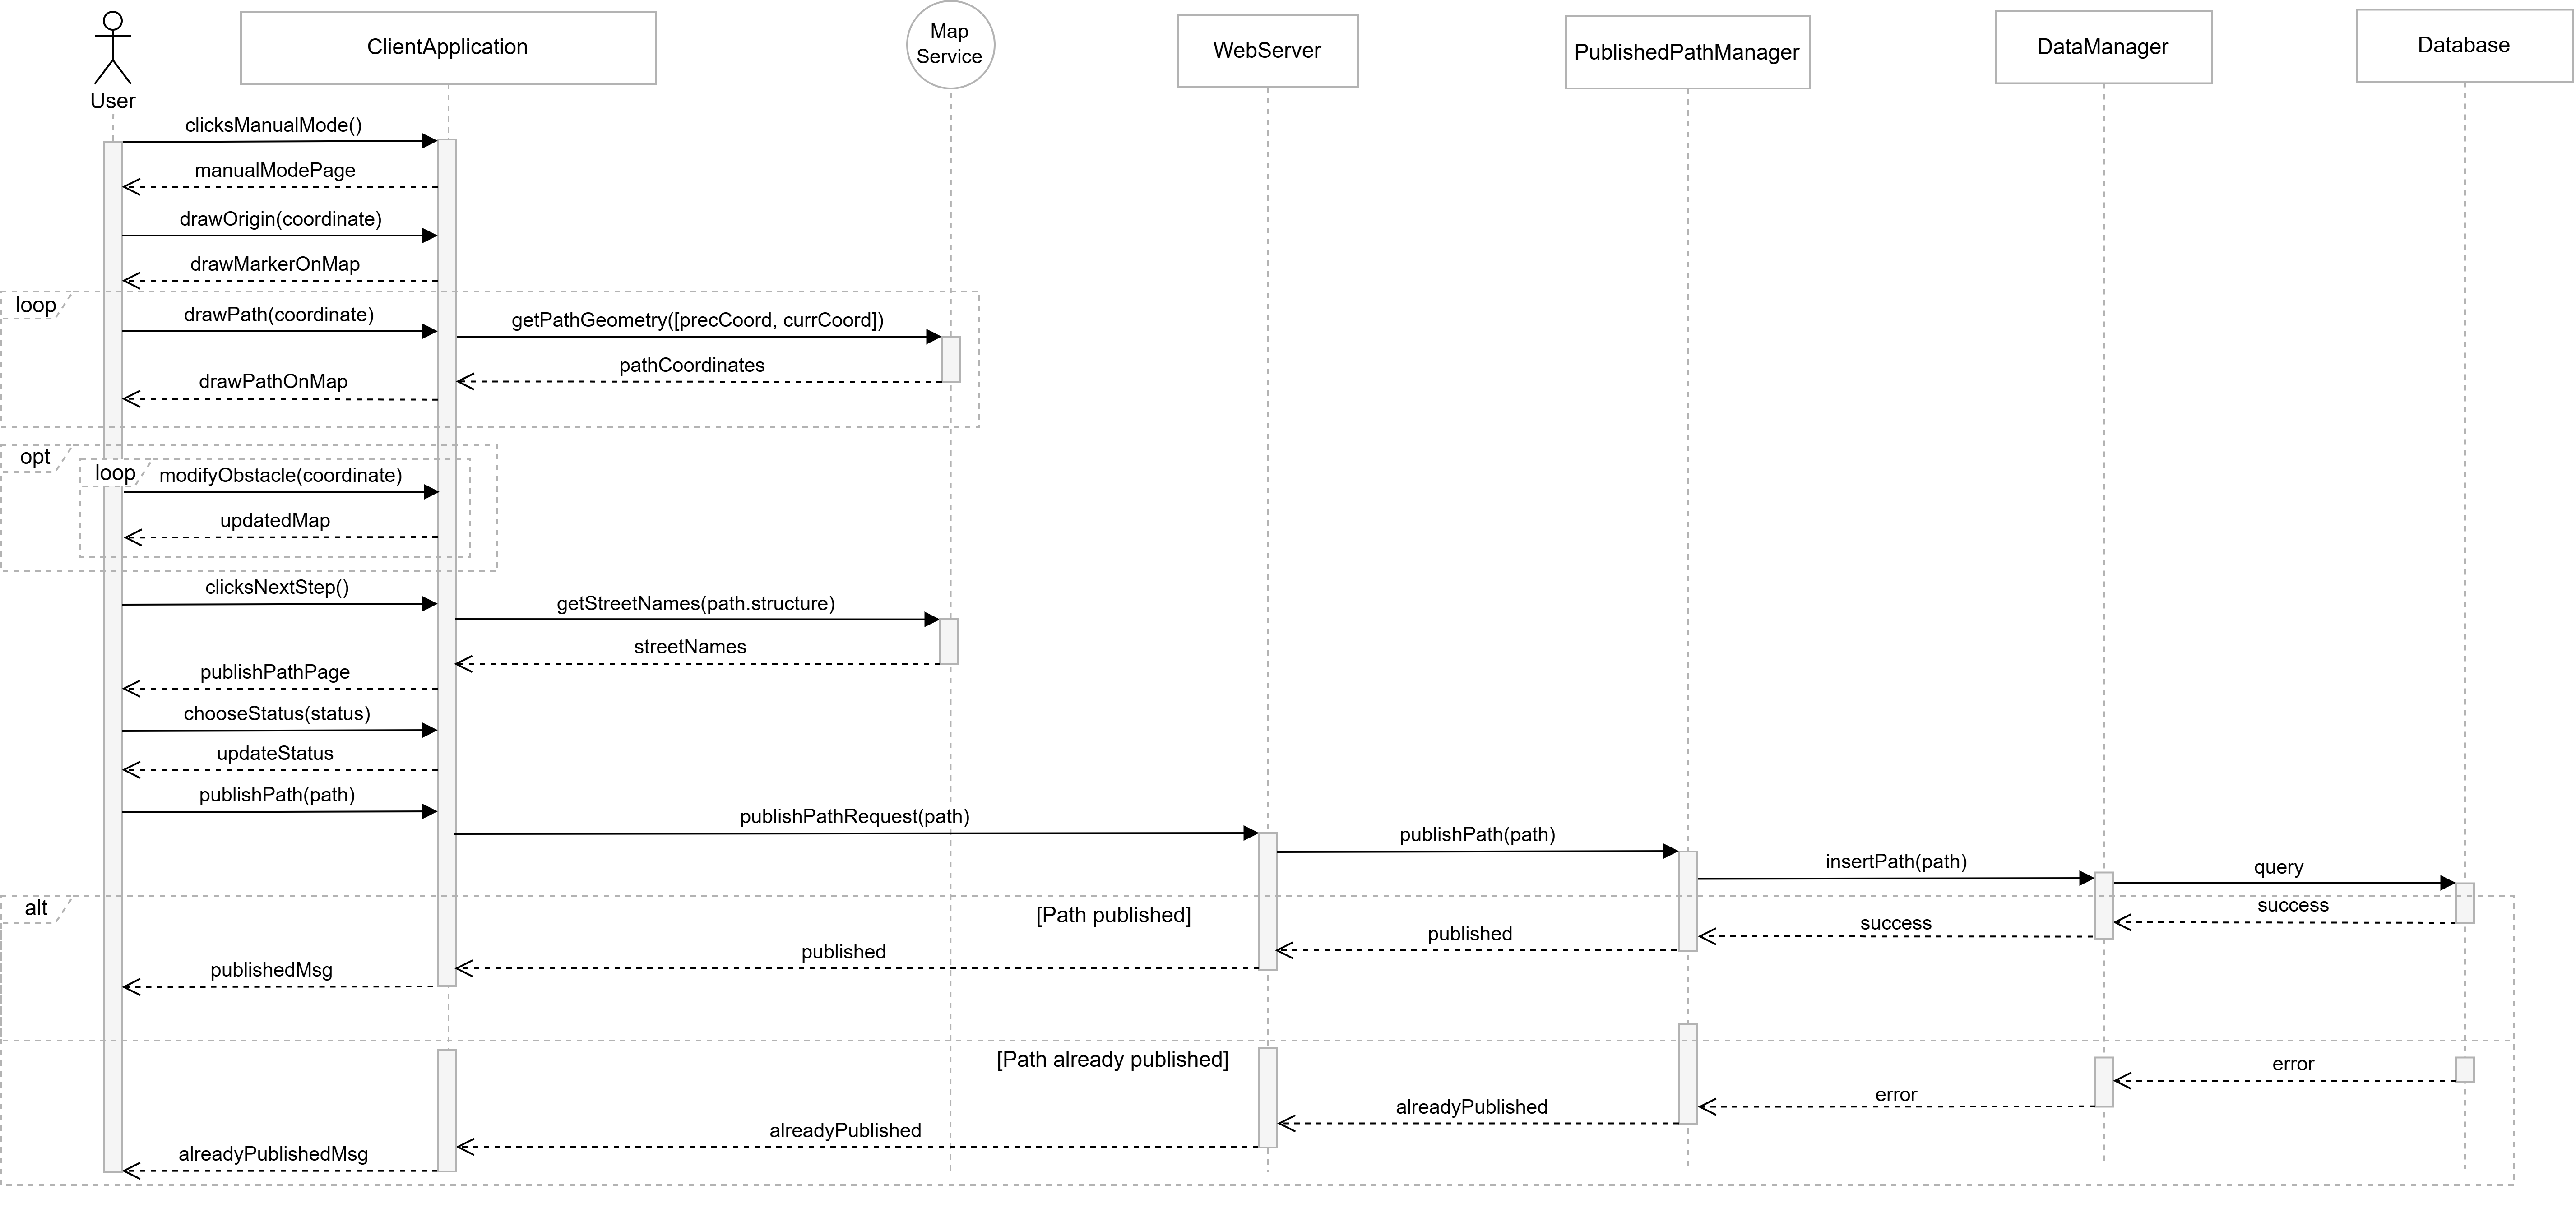
\includegraphics[width=1\linewidth]{DD//Images//SequenceDiagram/PublishPath.png}
    \caption{[SD9] Publish Path Sequence Diagram}
    \label{fig:placeholder}
\end{figure}

\noindent
This sequence diagram illustrates the manual path creation workflow. The user draws the path on the ClientApplication, which iteratively queries the external MapService to retrieve path geometry and street names. Distinctly, the obstacle tagging process is handled locally by the interface: the user can modify obstacles receiving immediate visual updates without triggering external service calls. Once finalized, the publication request is propagated through the WebServer and PublishedPathManager to the DataManager for persistence. The outcome is handled in an alternative block:
\begin{itemize}
    \item \textbf{Success:} The path is unique; the Database confirms insertion, and a success signal propagates back to notify the user.
    \item \textbf{Failure:} A duplicate path or error triggers a negative response, which is displayed to the user as an error message.
\end{itemize}



\newpage
\noindent
\textbf{[SD10] Automated Mode Sequence Diagram}
\begin{figure}[!h]
    \centering
         \includegraphics[width=1\linewidth]{DD/Images/SequenceDiagram/AutomatedMode.png}
    \caption{[SD10] Automated Mode Sequence Diagram}
    \label{fig:placeholder}
\end{figure}
\\
This sequence diagram describes the flow of the automatic activity recording mode. The User activates the automatic mode from the ClientApplication, which sends a start request to the WebServer. The WebServer delegates the operation to the AutomatedModeManager, which starts a timer and signals that the system is ready; the client then displays the automatic mode page. During the recording phase (loop block, while recording is active), the application collects data from the device sensors (gps, accelerometer, and gyroscope), sends these data to the AutomatedModeManager through the web server, and periodically receives the processing results and the elapsed time, which are displayed to the user in real time, with a small latency due to the data transmission time between client and server. The AutomatedModeManager checks for the presence of obstacles by analyzing accelerometer and gyroscope data, and computes activity metrics. When the user stops the automatic mode, the timer is stopped, the activity is marked as completed, and the client requests the weather from the Weather Service (through the web server and AutomatedModeManager) and the path geometry from the Map Service, so that they are already prepared for the display of the trip summary page, which is shown immediately afterward.


\newpage
\noindent
\textbf{[SD11] Publish Recorded Path Sequence Diagram}
\begin{figure}[!h]
    \centering
        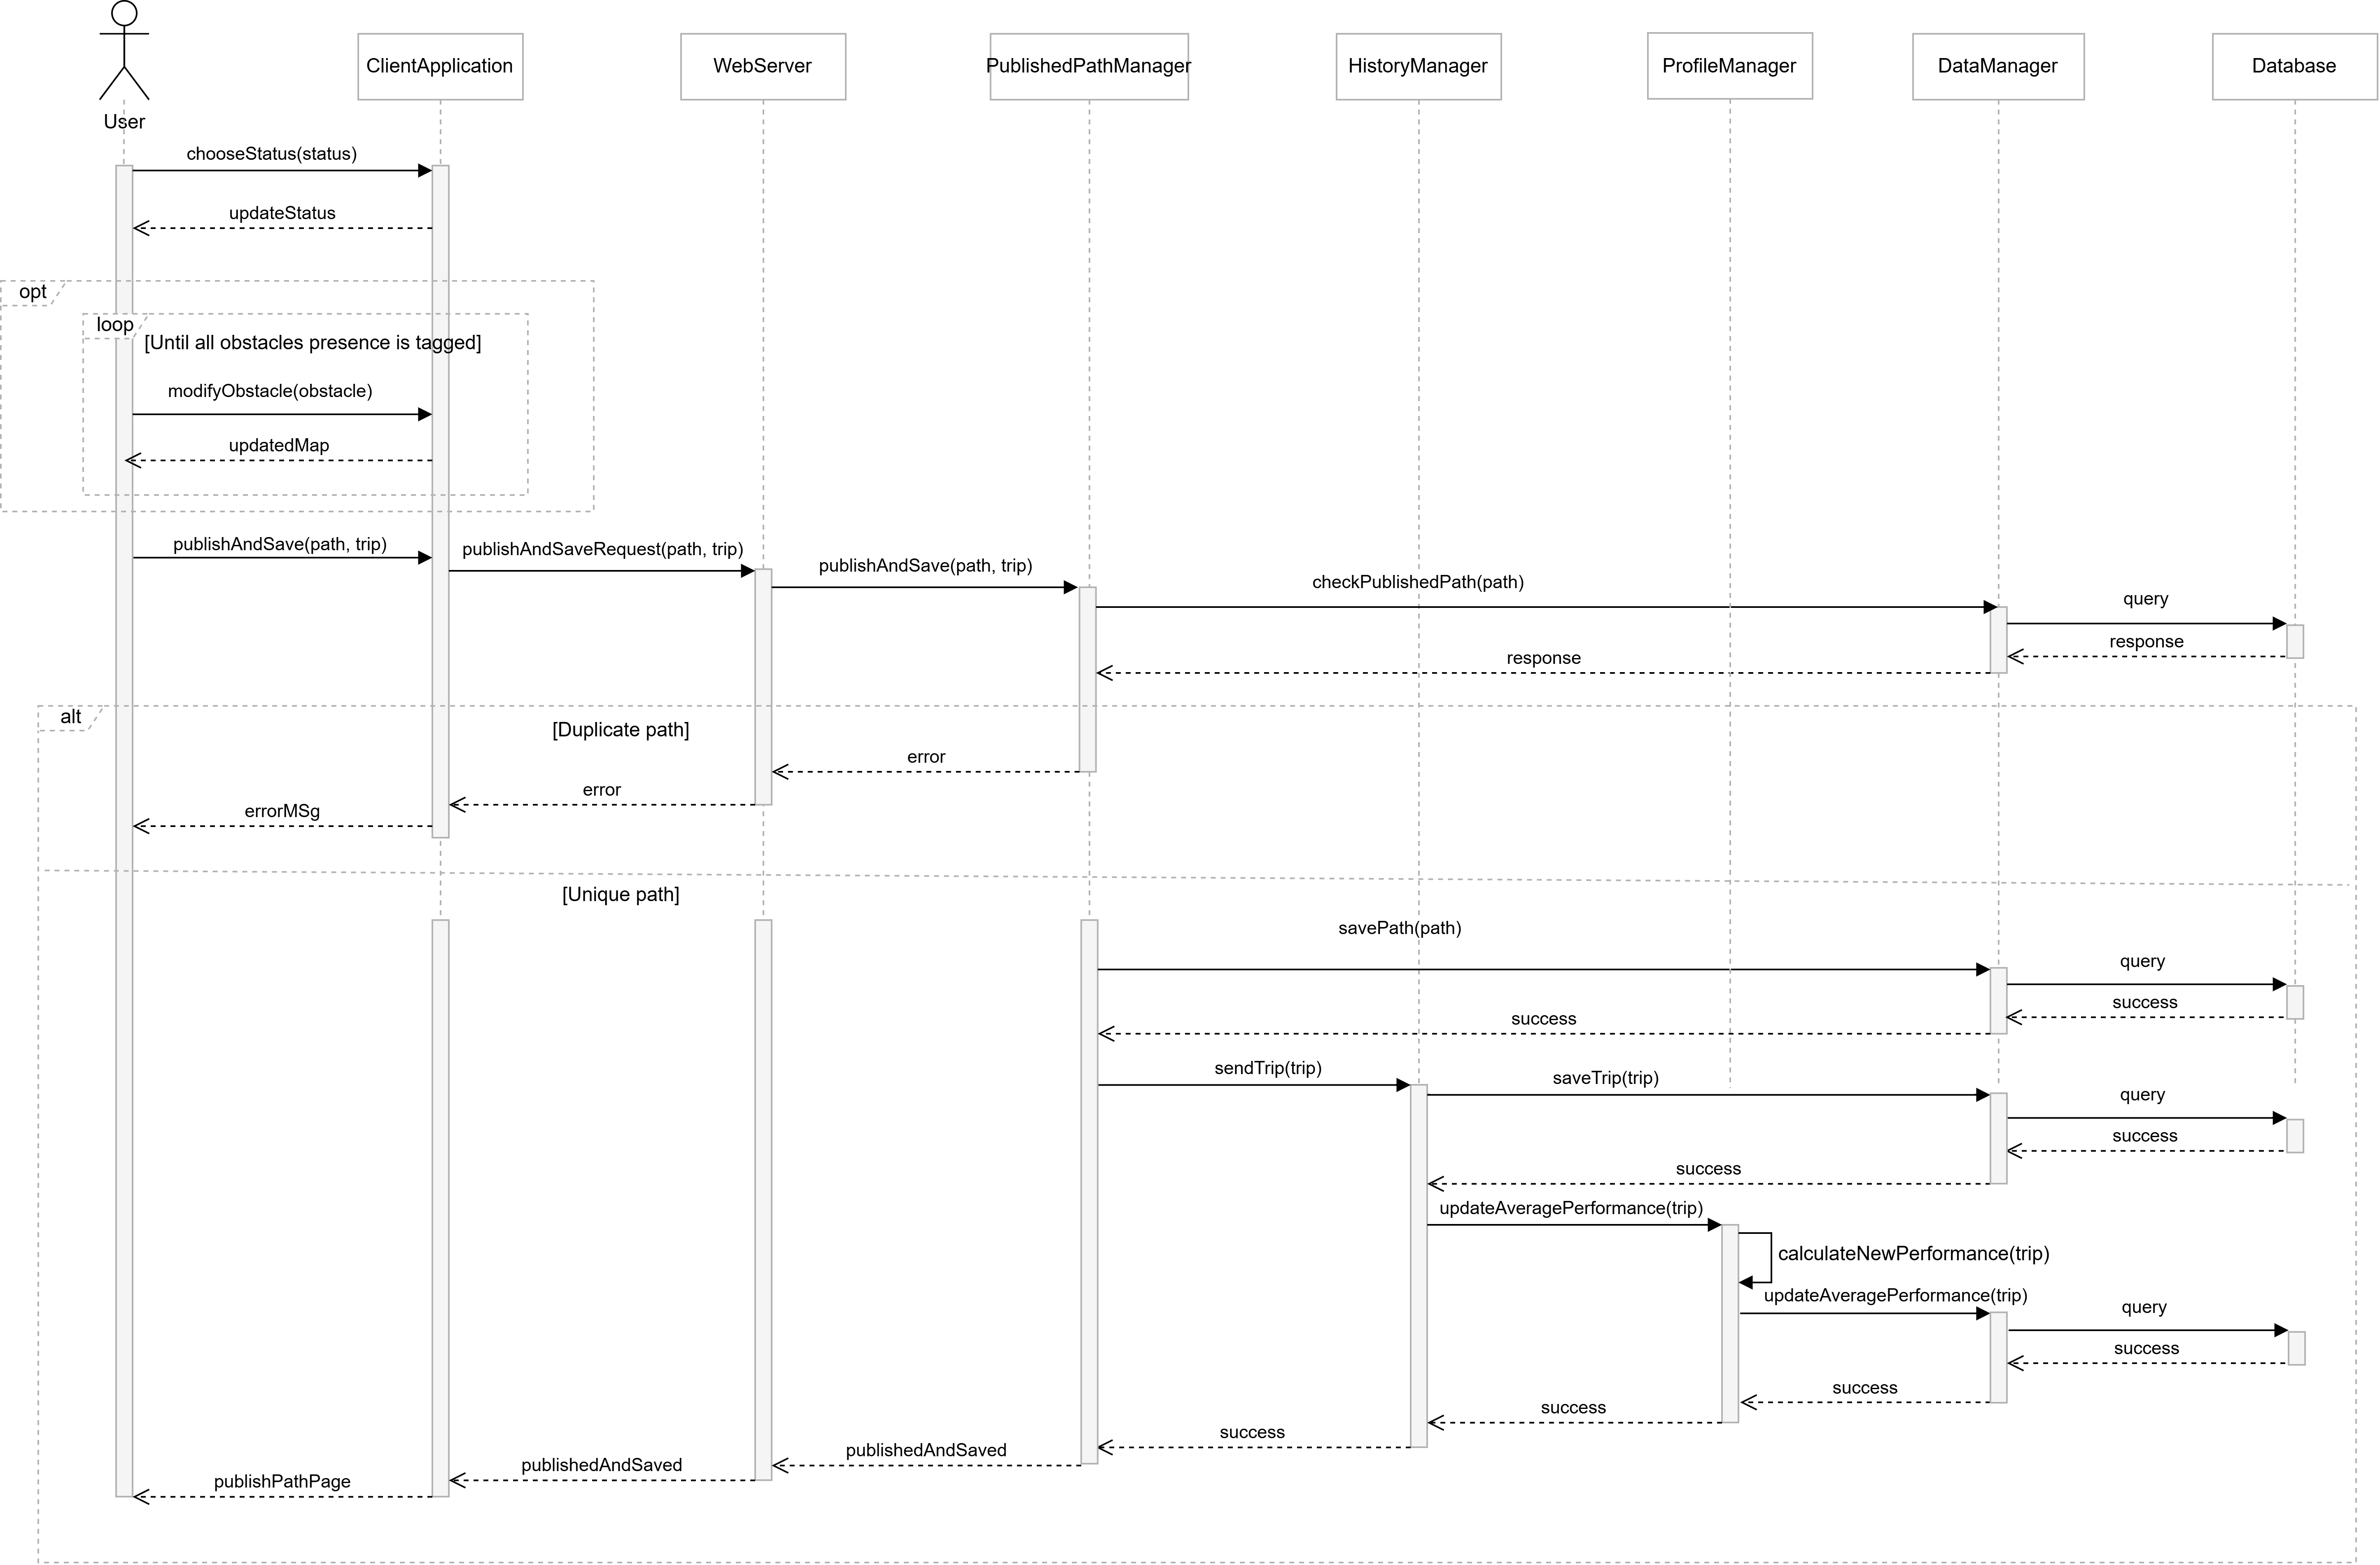
\includegraphics[width=1\linewidth]{DD/Images/SequenceDiagram/PublishRecordedPath.png}
    \caption{[SD11] Publish Recorded Path Sequence Diagram}
    \label{fig:placeholder}
\end{figure}
\\
 The process initiates with the user sets path status via the interface. An optional sequence, structured as a loop, allows the user to iteratively modify obstacle presence directly on the interface. Then, the user requesting to publish path and save a trip. This request is forwarded by the ClientApplication and WebServer to the PublishPathManager. Upon receiving the request, the PublishPathManager verifies the path's uniqueness by querying the DataManager. 

An alternative frame handles two distinct scenarios:
\begin{itemize}
    \item If the path already exists, the PublishPathManager returns an error, which propagates back through the system to the user as an error message.
    \item If the path is new, the system proceeds with a sequential persistence process. First, the PublishPathManager saves the path structure via the DataManager. Then, it delegates the trip details to the HistoryManager. The HistoryManager saves the trip data and subsequently triggers the ProfileManager to update the user's statistics. The ProfileManager calculates the new performance metrics and persists the updates via the DataManager. Only after all three operations (path, trip, and profile update) are confirmed, a success signal is returned and redirects user to publish path page.
\end{itemize}

\newpage
\subsection{Component Interface}
This section describes all service offered by the interface of each component.

\vspace{5mm}
\noindent
\textbf{Business tier}

\subsubsection{AccountManager Interfaces}
The AccountManager component exposes two interfaces: AccountServiceI, which is used by the WebServer, and AccountManagerI, which is used by the TripManager.\\
AccountServiceI methods:
\begin{itemize}
    \item \textbf{sendRegistration(user)}\\
    It returns a confermation link, indicating that the credentials have been successfully validated and triggering the start of the verification timer.
    \item \textbf{confermRegistrationEmail()}\\
    It returns a confirmation that the registration of guest in database was successful.
    \item \textbf{sendCredentials(email, pass)}\\
    It returns a confirmation of the validity of the provided credentials by querying the database.
    \item \textbf{modifyAccountInfo(email, accountInfo)}\\
    It returns a confirmation that the modification of account information in the database was successful.
\end{itemize}
AccountManagerI methods:
\begin{itemize}
    \item \textbf{updateAveragePerformance(trip)}\\
    It returns a confirmation that the update of the average performance metrics in the user's profile was successful.
\end{itemize}

\subsubsection{PathManager Interfaces}
The PathManager component exposes only the PathServiceI, which is used by the WebServer.\\
PathServiceI methods:
\begin{itemize}
    \item \textbf{searchPath(origin, dest)}\\
    It returns the top 5 paths based on the score.
    \item \textbf{deletePath(pathID)}\\
    It returns a confirmation that the deletion from the database was successful.
    \item \textbf{publishPath(path)}\\
    It returns a confirmation that the insertion in the database was successful.
    \item \textbf{startAutomatedMode()}\\
    It returns a confirmation that the automated mode is started.
    \item \textbf{sendInfo(currentPosition, accel, gyros)}\\
    It returns the processing result and the current timer value, derived after verifying the sensor data and calculating the trip metrics.
    \item \textbf{stopAutomatedMode()}\\
    It returns a confirmation that the automated mode is stopped.
    \item \textbf{publishAndSave(path, trip)}\\
    It returns a confirmation indicating that the path has been successfully published and the associated trip saved.
\end{itemize}

\subsubsection{TripManager Interfaces}
The TripManager component exposes two interfeces: TripServiceI, which is used by the WebServer, and TripManangerI, which is used by the PathManager.\\
TripServiceI methods:
\begin{itemize}
    \item \textbf{startNavigation()}\\
    It starts the internal navigation timer and returns a positive status indicating the system is ready to track the user.
    \item \textbf{metrics(path, currentPosition)}\\
    It starts the cyclist position checking and the metrics calculation up to now, returns the current speed.
    \item \textbf{weatherInfo(List<coordinate>)}\\
    It returns a collection of meteorological data, providing weather details for every coordinate in the provided list.
    \item \textbf{saveJourney(trip, report)}\\
    It returns a signal confirming that both the trip data and the associated report have been successfully persisted in the system.
    \item \textbf{recentTrips(email)}\\
    It returns the list of trips recently completed by the specified user, retrieved via the DataManager.
    
\end{itemize}
TripManagerI methods:
\begin{itemize}
    \item \textbf{sendTrip(trip)}\\
    It returns a confirmation indicating that the trip details have been successfully persisted by the DataManager.
\end{itemize}
\subsubsection{ReportManager Interfaces}
The ReportManager component exposes only the ReportManagerI, which is used by TripManager.\\
ReportManagerI methods:
\begin{itemize}
    \item \textbf{sendReport(report)}\\
    It returns a confirmation indicating that the report has been successfully saved.
\end{itemize}

\subsubsection{DataManager Interfaces}
The DataManager component exposes only the DataManagerI, which is used by all components of Business Tier: AccountManager, ReportManager, PathManager, TripMananger.\\
DataManagerI methods:
\begin{itemize}
    \item \textbf{checkCredentials(user)}\\
    it returns a confirmation that the credentials are valid and that the user does not already exist in the database.
    \item \textbf{insert(user)}\\
    it returns a confirmation that the insertion of the user's registration information into the database was successful.
    \item \textbf{checkCredentials(email, pass)}\\
    it returns a confirmation that the provided email and password are correct and exist in the database.
    \item \textbf{getBestPaths(origin, dest)}\\
    It returns the top 5 paths stored in the database that match the corresponding origin and destination, ranked based on their score.
    \item \textbf{saveTrip(trip)}\\
    It returns a confirmation indicating that the trip details have been successfully persisted in the database.
    \item \textbf{saveReport(report)}\\
    It returns a confirmation indicating that the report details have been successfully persisted in the database.
    \item \textbf{updateAveragePerformance(trip)}\\
    It returns a confirmation indicating that the user's performance statistics have been recalculated based on the new trip details and successfully updated in the database.
    \item \textbf{getRecentTrips(email)}\\
    It returns the raw data of the past trips performed by the user, fetched from the database.
    \item \textbf{putAccountInfo(email, accountInfo)}\\
    It returns a success confirmation indicating that the account information associated with the specified user has been successfully updated in the database.
    \item \textbf{deletePath(pathID)}\\
    It returns a confirmation indicating that the path associated with the specified ID has been successfully removed from the database.
    \item \textbf{insertPath(path)}\\
    It returns a confirmation indicating that the new path details have been successfully inserted and persisted in the database.
    \item \textbf{checkPublishedPath(path)}\\
    It returns the existence status of the path to prevent the creation of duplicate entries.
    \item \textbf{savePath(path)}\\
    It returns a success signal acknowledging that the new path definition has been correctly stored.
\end{itemize}

\newpage
\vspace{5mm}
\noindent
\textbf{Data tier}

\subsubsection{Database Interfaces}
The Database component exposes the DBMS API, which is utilized by the DataManager to execute queries on the database and retrieve the results.


\vspace{5mm}
\noindent
\textbf{Web tier}

\subsubsection{WebServer Interfaces}
The WebServer component exposes only the WebServerI, which is used by the ClientApplication.\\
WebServerI methods:
\begin{itemize}
    \item \textbf{sendRegistrationRequest(user)}\\
    This request is forwarded to the RegistrationManager and returns a confirmation indicating that the system has successfully validated the credentials and sent the verification link.
    \item \textbf{confermRegistrationEmailRequest()}\\
    This request is forwarded to the RegistrationManager and returns a confirmation that the registration process was successful.
    \item \textbf{sendCredentialsRequest(email, pass)}\\
    This request is forwarded to the AuthMananger and returns a confirmation that all provided credential are correct and exist in the database.
    \item \textbf{searchPathRequest(origin, dest)}\\
    This request is forwarded to the SearchPathManager and returns the top 5 best-scored paths with correspond origin and destination.
    \item \textbf{startNavigationRequest()}\\
    This request is forwarded to the NavigationManager and returns a confirmation that the NavigationManager is ready.
    \item \textbf{metricRequest(path, currentPosition)}\\
    This request is forwarded to the NavigationManager and returns the current street and the current speed.
    \item \textbf{weatherInfoRequest(List<coordinate>)}\\
    This request is forwarded to the NavigationManager, which, through the ExternalProxy, requests weather information related to the path from the Weather Service. In particular, The Weather Service returns the weather condition that occurs most frequently among the provided coordinates.
    \item \textbf{saveJourneyRequest(trip, report)}\\
    This request is forwarded to the HistoryManager and returns a confirmation that trip and report were saved in the database.
    \item \textbf{recentTripsRequest(email)}\\
    This request is forwarded to the HistoryManager and returns the recent trips list.
    \item \textbf{modifyAccountInfoRequest(email, accountInfo)}\\
    This request is forwarded to the ProfileManager and returns a confirmation that the update account information process was successful.
    \item \textbf{deletePathRequest(pathID)}\\
    This request is forwarded to the PublishedPathManager and returns a confirmation that the deletion process was successful.
    \item \textbf{publishPathRequest(path)}\\
    This request is forwarded to the PublishedPathManager and returns a confirmation that the publication process was successful.
    \item \textbf{startAutomatedModeRequest()}\\
    This request is forwarded to the AutomatedModeManager and returns a confirmation that the AutomatedModeManager is ready.
    \item \textbf{sendInfoRequest(currentPosition, accel, gyros)}\\
    This request is forwarded to the AutomatedModeManager and returns the total distance covered, the current and average speed, a boolean value represents the presence of an obstacle, and the timer value.
    \item \textbf{stopAutomatedModeRequest()}\\
    This request is forwarded to the AutomatedModeManager and returns all the information related to the traveled path.
    \item \textbf{publishAndSaveRequest(path, trip)}\\
    This request is forwarded to PublishPathManager and returns a confirmation that the new path being published and the trip details being securely stored in the database.
\end{itemize}

\subsubsection{ExternalProxy Interfaces}
The ExternalProxy exposes the ExternalServicesI interface, enabling components within the system to utilize the services provided by the MapService and WeatherService.\\
ExternalServicesI methods:
\begin{itemize}
    \item \textbf{getWeatherInfo(List<coordinate>)}\\
    This request is forwarded to the Weather Service and returns the weather information for all the coordinates provided.
\end{itemize}

\newpage
\vspace{5mm}
\noindent
\textbf{Presentation tier}\\
\subsubsection{ClientApplication Interfaces}
The ClientApplication component exposes the UserAppI, which is used by the cyclists.\\
UserAppI methods:
\begin{itemize}
    \item \textbf{enterAccountInfo(user)}\\
    It initiates the registration sequence by submitting the user's credentials. In the success scenario, this triggers the backend validation process which results in the system sending a verification email.
    \item \textbf{confermEmail()}\\
    it submits the user's registration details. Upon successful completion, the guest is redirected to the login page.
    \item \textbf{enterCredentials(email,pass)}\\
    it submits the user's credentials. Upon successful completion, the guest is redirected to the account page.
    \item \textbf{enterDestination(dest)}\\
    It returns the map on which the paths with the corresponding origin and destination are drawn.
    \item \textbf{enterOrigin(origin)}\\
    It updates the internal state of the ClientApplication with the origin selected by the user, preparing the data for the navigation.
    \item \textbf{clicksStartNavigation()}\\
    It triggers the navigation initialization sequence, resulting in the cyclist being redirected to the navigation interface once the system is ready. 
    \item \textbf{chooseStatus(status)}\\
    It updates the internal state of the ClientApplication with the status selected by the user, preparing the data for the trip report.
    \item \textbf{modifyObstacle(obstacle)}\\
    It updates the local status of a specific obstacle and immediate refresh of the map display.
    \item \textbf{saveTripAndReport(trip, report)}\\
    It initiates the final save operation for the completed trip and its associated report, ultimately redirecting the user to the home page.
    \item \textbf{clicksRecentTrips(email)}\\
    It redirects user to recent trip page upon success.
    \item \textbf{modifyAccountInfo(email, accountInfo)}\\
    It returns a confirmation indicating that the valid account information has been accepted and successfully updated in the database.
    \item \textbf{deletePath(pathID)}\\
    It returns a confirmation indicating that the path associated with the specified ID has been successfully removed from the database.
    \item \textbf{clicksManualMode()}\\
    It redirects the user to manual mode page.
    \item \textbf{drawOrigin(coordinate)}\\
    It represents the user's interaction to define the starting point of the path on the map, which triggers the application to display a marker at the selected coordinate.
    \item \textbf{drawPath(coordinate)}\\
    It allows the user to extend the path by adding new marker, triggers the application to calculate the connecting geometry and update the visual representation of the path on the map.
    \item \textbf{publishPath(path)}\\
    It triggers the storage of the manually created path into the database via the PublishedPathManager, confirming the permanent addition of the new path.
    \item \textbf{clicksAutomatedMode()}\\
    It triggers the start of the automated recording session, resulting in the system initialization and the transition to the automated mode page.
    \item \textbf{stopAutomatedMode()}\\
    It ends the automated tracking process and redirects the user to the trip summary page to view the recorded path details.
    \item \textbf{publishAndSave(path, trip)}\\
    It triggers a sequence that validates the path against existing records. Upon successful validation, it sequentially saves the path structure and the trip history to the database before confirming the operation to the user.
    \item \textbf{getMapData()}\\
    This request is forwarded to the Map Service and returns the necessary metadata that allow the ClientApplication to initialize its local mapping engine and use graphical libraries.
    
\end{itemize}

\vspace{5mm}
\noindent
\textbf{External Services}

\subsubsection{MapService Interfaces}
The external Map service exposes the MapServiceI, which is used by ExternalProxy.\\
MapServiceI methods:
\begin{itemize}
    \item \textbf{currentStreet(currentPosition)}\\
    It returns the name of the street corresponding to the current position, retrieved from the external Map Service.
    \item \textbf{getPathGeometry(List<coordinate>)}\\
    It returns the detailed coordinates of the path, retrieved from the external Map Service, based on the provided list of coordinates of markers.
    
\end{itemize}

\subsubsection{WeatherService Interfaces}
The WeatherService exposes the WeatherServiceI, which is used by ExternalProxy.\\
WeatherServiceI methods:
\begin{itemize}
    \item \textbf{getWeatherInfo(List<coordinate>)}\\
    It returns a list of weather conditions, each one associated with one coordinate in the list passed as a parameter.
\end{itemize}

\subsubsection{Sensors Interfaces}
The Sensors exposes the SensorsI, which is used by ClientApplication.\\
Sensors methods:
\begin{itemize}
    \item \textbf{getCurrentPosition()}\\
    It returns the current location data detected by the device's GPS.
    \item \textbf{getSensorsData()}\\
    It returns the real-time telemetry data, specifically the current position, accelerometer readings, and gyroscope values, retrieved directly from the device's sensors.
\end{itemize}

\subsection{Selected Architectural Styles and Patterns}
\noindent
This section describes the architectural styles and design patterns selected for the Best Bike Paths (BBP) system, providing the rationale for their adoption in terms of scalability, security, and maintainability.
The System is organized according to a robust and highly scalable architectural style for distributed applications: the Client-Server architecture with four tiers.
\begin{itemize}
    \item \textbf{Presentation Tier}\\
    It consists of application clients that make requests to the application server through the web server. It communicates with the map service and manages all graphical interactions with the user.
    \item \textbf{Web Tier}\\
    This is the DMZ of the system. It consists of components that handle the interaction between the clients and the business logic. It includes the Web Server, which acts as the primary entry point for all incoming traffic, managing the logical routing of requests. Additionally, this tier hosts the External Proxy, a specialized component that manages outbound communication with third-party APIs (weather services). This ensures that the internal network remains isolated.
    \item \textbf{Business Tier}\\
    It consists of components that provide the core business logic for the application. It processes the raw data coming from the Web Tier and coordinates data persistence toward the Data Tier.
    \item \textbf{Data Tier}\\
    It consists of the database server and the DBMS. This layer handles the persistence of all information, which are accessed exclusively by components in the business tier through secure connections.
\end{itemize}

\subsection{Other Design Decisions}
\begin{itemize}
    \item \textbf{Master-slave database architecture}\\
    The Master–Slave architecture centralizes write operations on a single node (the master), while distributing read operations across multiple synchronized replicas (slaves) to optimize performance. The master is responsible for handling all write requests and propagating updates to the slaves to keep them consistent. This structure ensures service continuity even in the event of a failure of the primary server.
    \item \textbf{daily report merging}\\
    Every day at midnight, the daily reports are merged, and the information of the corresponding paths is subsequently updated.\\
    \item \textbf{direct communication of the ClientApplication with the Map Service}\\
    For performance reasons, crucial, for example, for communicating the name of the current street during navigation, the ClientApplication communicates directly with the Map Service, without passing through the Application Server. server.
    \item \textbf{No calculation requests are sent to the Map Service}\\
    Only the map and the graphical libraries are requested from the Map Service; all calculations, such as checking whether the cyclist is on the route during navigation, are handled by the Application Server. This approach is adopted to remain as independent as possible from external services, requesting only the minimum necessary.
\end{itemize}

\newpage